\documentclass[conference]{IEEEtran}

% ====== Paquetes ======
\usepackage[utf8]{inputenc}
\usepackage[T1]{fontenc}
\usepackage[spanish,es-nodecimaldot,es-noshorthands]{babel}
\usepackage{graphicx}
\usepackage{amsmath, amssymb}
\usepackage{cite}
\usepackage{float}
\usepackage{placeins}
\usepackage{url}
\usepackage{xcolor}
\usepackage{booktabs}
\usepackage{multirow}
\usepackage{tikz}
\usetikzlibrary{positioning, shapes.geometric, arrows.meta, calc}
\usepackage{hyperref}
\hypersetup{hidelinks}
\graphicspath{{figs/}}
\raggedbottom

% ====== Datos del artículo ======
\title{Laboratorio 5 - Control en discreto de un sistema mecánico}

\author{
    \IEEEauthorblockN{
        Juan Sebastian Muñoz (7004437), \quad
        José Miguel Gómez Urbina (7004416),\\
        Sergio Alejandro Contreras (7004444)\\
    }
    \IEEEauthorblockA{
        Ingeniería Mecatrónica\\
        Universidad Militar Nueva Granada\\
        Bogotá D.C., Colombia\\
        \texttt{est.juans.munozg@unimilitar.edu.co},
        \texttt{est.josem.gomezu@unimilitar.edu.co} \\
        \texttt{est.sergioa.contre1@unimilitar.edu.co} \\ }
    }

\begin{document}

\maketitle

% ================= ABSTRACT =================
\begin{abstract}
En este documento se presenta el diseño, la simulación y la implementación de
dos controladores discretos para la posición de un sistema mecánico
piñón--cremallera con resortes, accionado por un motor DC mediante un puente H
L298N y medido con un encoder incremental. La planta se caracterizó en lazo
abierto y se identificó como un sistema de segundo orden con zona muerta
asimétrica por fricción estática. A partir del modelo se obtuvo la función de
transferencia de pulso con retenedor de orden cero y $T=10$~ms. Se diseñaron
un PID por asignación de polos discretizado por Euler hacia atrás (técnica
continuo--discreto) y un controlador con integrador diseñado directamente en
el plano $z$ (técnica discreto--discreto), con el mismo polinomio deseado. Ambos
se validaron en MATLAB/Simulink considerando la saturación del actuador y la
cuantización del encoder, se implementaron como ecuaciones en diferencias en
un ESP32 y se evaluaron con una interfaz gráfica que calcula el índice ISE en
tiempo real. En la planta real ambos controladores siguen la referencia con un
error final de $\pm0.10$~mm (1.5 cuentas del encoder); el continuo--discreto
fue más rápido y con menor ISE, mientras que el discreto--discreto exigió
menos acción de control.
\end{abstract}

\begin{IEEEkeywords}
Control digital, discretización, retenedor de orden cero, PID discreto,
asignación de polos, ecuación en diferencias, ISE, ESP32, sistema mecánico.
\end{IEEEkeywords}

% ================= INTRODUCCIÓN =================
\section{Introducción}

El control digital reemplaza el controlador analógico por un algoritmo que se
ejecuta en un procesador a intervalos fijos de tiempo: la salida de la planta
se muestrea, se convierte a un número, se calcula la acción de control y esta
se mantiene constante hasta la siguiente muestra \cite{ogata1995, franklin1998}.
Existen dos caminos para diseñar el controlador discreto: diseñar en tiempo
continuo y luego discretizar el controlador (técnica continuo--discreto), o
discretizar primero la planta y diseñar directamente en el plano $z$ (técnica
discreto--discreto) \cite{ogata1995}.

En la práctica 3 se controló la posición del mismo tipo de sistema mecánico
con un PID analógico construido con amplificadores operacionales. En esta
práctica la planta se reemplazó por un sistema piñón--cremallera con dos
resortes, se volvió a identificar su modelo y los controladores se
implementaron en un microcontrolador ESP32 \cite{espressif2024}, con una
interfaz gráfica para cambiar la referencia, graficar las señales y calcular
el índice de error cuadrático integrado (ISE).

\subsection{Objetivos}
\begin{itemize}
  \item Diseñar un PID continuo y discretizarlo (técnica continuo--discreto).
  \item Diseñar un controlador a partir de la planta discretizada (técnica
        discreto--discreto).
  \item Evaluar ambos mediante el ISE y los parámetros de la respuesta.
  \item Implementarlos en un microcontrolador sobre el sistema mecánico.
\end{itemize}

% ================= MARCO TEÓRICO =================
\section{Marco teórico}

\subsection{Métodos de discretización}
Discretizar consiste en aproximar una función de transferencia $F(s)$ por una
$F(z)$ con periodo de muestreo $T$. Los métodos más usados son
\cite{ogata1995, franklin1998}:
\begin{enumerate}
  \item \textbf{Euler hacia adelante}, $s \approx (1-z^{-1})/(Tz^{-1})$. Es el
        más simple, pero puede convertir un sistema estable en inestable si $T$
        es grande. Se usa para integrar numéricamente la velocidad de un robot
        móvil a partir de la odometría.
  \item \textbf{Euler hacia atrás}, $s \approx (1-z^{-1})/T$. Siempre conserva
        la estabilidad y es la forma habitual de los PID en controladores
        lógicos programables (PLC) que regulan temperatura o caudal.
  \item \textbf{Tustin o bilineal},
        $s \approx \frac{2}{T}\frac{1-z^{-1}}{1+z^{-1}}$. Conserva la
        estabilidad y la respuesta en frecuencia hasta cerca de la frecuencia
        de Nyquist; se usa en filtros digitales de audio y en los lazos de
        corriente de variadores de motores.
  \item \textbf{Retenedor de orden cero (ZOH)},
        $G(z) = (1-z^{-1})\,\mathcal{Z}\{G(s)/s\}$. Da el equivalente exacto de
        una planta excitada por una señal escalonada, como el PWM de un
        convertidor; se usa para discretizar plantas en control de posición de
        servomotores y en este laboratorio.
  \item \textbf{Mapeo de polos y ceros}, $z = e^{sT}$ para cada polo y cero,
        ajustando la ganancia DC; se usa al trasladar compensadores de adelanto
        y atraso en sistemas de vuelo.
\end{enumerate}

\subsection{Selección del tiempo de muestreo}
\textbf{Criterio por el tiempo de establecimiento.} $T$ se toma como una
fracción de $t_s$: entre $t_s/10$ y $t_s/20$ cuando se diseña el lazo cerrado,
y entre $t_s/40$ y $t_s/80$ cuando se muestrea la planta en lazo abierto. Por
ejemplo, un horno con $t_s\approx 20$~min admite $T$ de 1~min, mientras que un
lazo de posición de un disco duro con $t_s$ de pocos milisegundos exige
$T$ de decenas de microsegundos.

\textbf{Criterio de Landau.} Para un par dominante con frecuencia natural
$\omega_n$ y $0.7 \le \zeta \le 1$, $0.25 \le \omega_n T \le 1.5$
\cite{landau2006}. Un brazo robótico con $\omega_n = 10$~rad/s admite
$25~\text{ms} \le T \le 150$~ms; un dron con $\omega_n = 60$~rad/s en el lazo
de actitud requiere $T \le 25$~ms (en la práctica se usan 2--4~ms por el ruido).

\subsection{Ecuación en diferencias}
Es la relación entre la salida en el instante $k$ y valores actuales y
pasados de la entrada y la salida; es el equivalente discreto de una ecuación
diferencial. Si un controlador es
\begin{align*}
  \frac{U(z)}{E(z)} = \frac{q_0+q_1z^{-1}+q_2z^{-2}}{1+p_1z^{-1}+p_2z^{-2}},
\end{align*}
se multiplica en cruz y se usa que $z^{-n}X(z)$ corresponde a $x(k-n)$:
\begin{align*}
  u(k) &= -p_1u(k-1) - p_2u(k-2)\\
       &\quad + q_0e(k) + q_1e(k-1) + q_2e(k-2).
\end{align*}
En un microcontrolador o una tarjeta de adquisición se programa con una
interrupción o tarea periódica de periodo $T$: se lee el sensor, se evalúa la
ecuación con variables que guardan los valores anteriores, se escribe la
salida (PWM o DAC) y se desplazan las variables una posición \cite{franklin1998}.

\subsection{Retenedor de orden cero}
Es el elemento que convierte la secuencia de números $u(k)$ en una señal
continua, manteniendo cada valor constante durante un periodo:
$G_{ZOH}(s) = (1 - e^{-sT})/s$. En un microcontrolador lo implementan el DAC o
el registro de PWM, que no cambian hasta la siguiente actualización. Por eso la
planta vista por el controlador es $(1-z^{-1})\,\mathcal{Z}\{G(s)/s\}$
\cite{ogata1995}.

% ================= DESARROLLO =================
\section{Desarrollo}

\subsection{Montaje}
La planta es una cremallera de masa $M$ sujeta por dos resortes $k_1$, $k_2$,
movida por un piñón de radio $r=9.4$~mm acoplado a un motor DC con reducción
20:1 (Fig.~\ref{fig:montaje}). El motor se maneja con un puente H L298N con
PWM de 1~kHz, y la posición se mide con el encoder del motor (11 pulsos por
vuelta) leído en cuadratura x4 por el contador de pulsos del ESP32, lo que da
una resolución de
\begin{align*}
  \Delta x = \frac{2\pi(9.4)}{11\cdot 20\cdot 4} = 0.0671~\text{mm/cuenta}.
\end{align*}
La posición al encender es el cero y la derecha es el sentido positivo.

\begin{figure}[!htb]
  \centering
  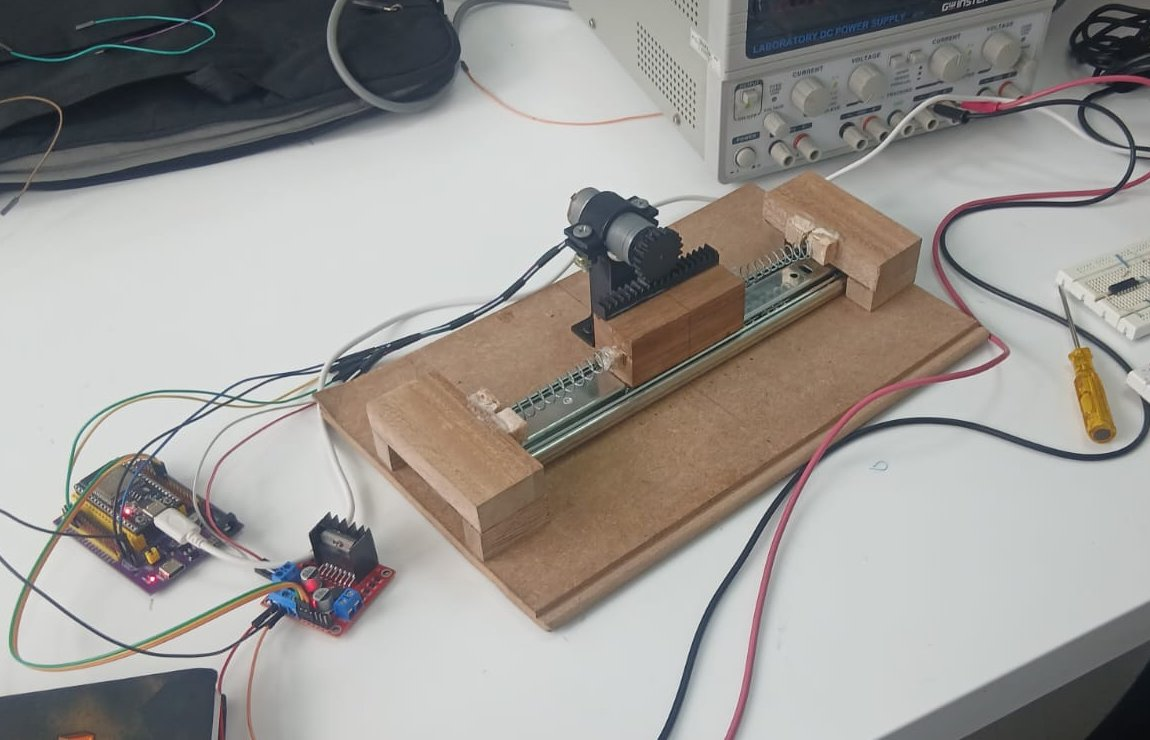
\includegraphics[width=\linewidth]{montaje.jpg}
  \caption{Montaje físico: cremallera con resortes sobre la guía, motor DC con
  encoder y piñón, ESP32, puente H L298N y fuente de laboratorio.}
  \label{fig:montaje}
\end{figure}

\subsection{Caracterización}
En reposo, el encoder no mostró ruido ni deriva (0 cuentas durante 2~s). Con
pulsos de PWM a ambos lados (Fig.~\ref{fig:carac}) se observó que:
\begin{itemize}
  \item Al 100~\% la masa llega a un equilibrio contra los resortes de
        $+15.8$~mm a la derecha y $-14.6$~mm a la izquierda en unos 220~ms; este
        es el recorrido máximo que el motor puede sostener.
  \item Al soltar el motor la masa vuelve oscilando y queda a $\pm1$~mm del
        cero por fricción y juego del piñón.
  \item Hay una zona muerta grande: por debajo de $\approx50~\%$ de PWM la masa
        no se mueve desde el reposo, y el sistema presenta stick--slip.
\end{itemize}

\begin{figure}[!htb]
  \centering
  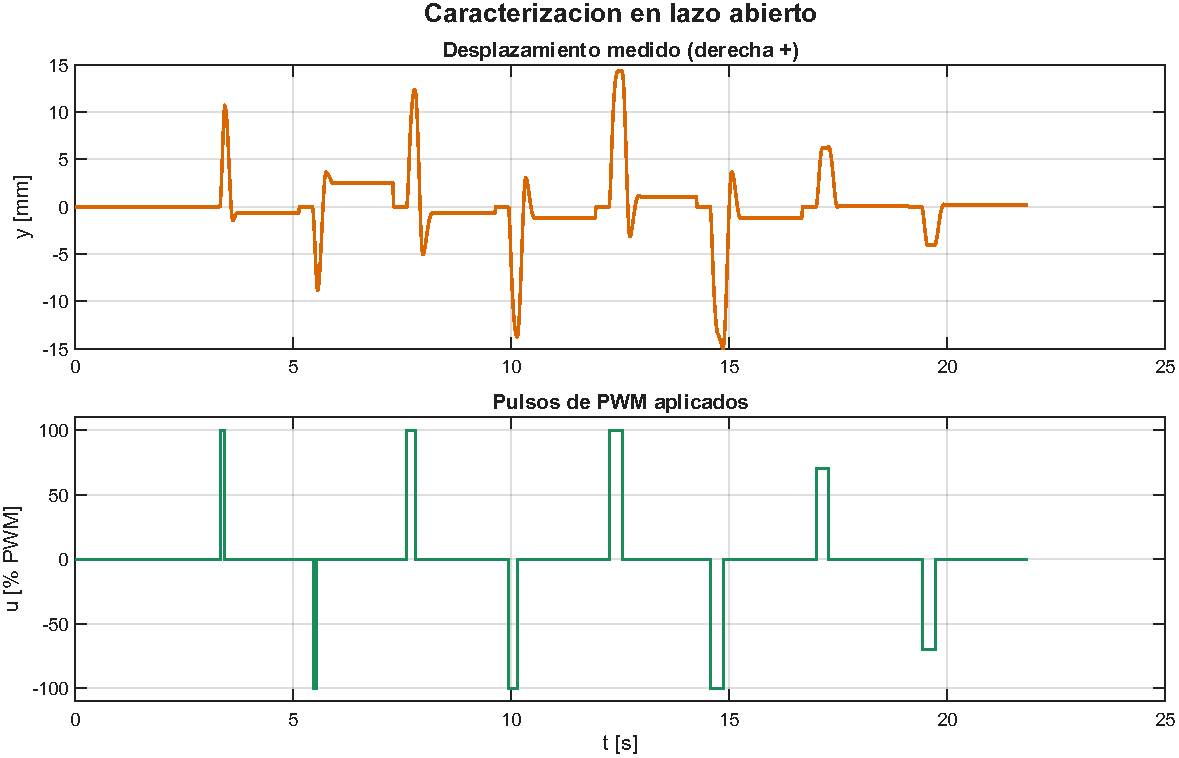
\includegraphics[width=\linewidth]{caracterizacion.pdf}
  \caption{Pulsos de PWM en lazo abierto y desplazamiento medido.}
  \label{fig:carac}
\end{figure}

\subsection{Identificación}
Se aplicaron diez escalones ($\pm60$ a $\pm100~\%$) desde el reposo. La recta
que ajusta el equilibrio contra el PWM (Fig.~\ref{fig:eq}) da la zona muerta de
cada lado: $u_0^+ = 42.1~\%$ y $u_0^- = 55.3~\%$. Con la entrada efectiva
$u_{ef} = \operatorname{sign}(u)\max(|u|-u_0, 0)$ y estimación con
\texttt{tfest} sobre todos los escalones a la vez (Fig.~\ref{fig:ajuste}):
\begin{equation}
  G(s) = \frac{Y(s)}{U_{ef}(s)} = \frac{168.4}{s^2 + 46.87\,s + 622.9}
  \quad\left[\frac{\text{mm}}{\%}\right]
  \label{eq:Gs}
\end{equation}
con $\omega_n = 24.958$~rad/s, $\zeta = 0.939$, $K = 0.2703$~mm/\%, polos
$s = -23.435 \pm j8.585$ y $t_s = 4/(\zeta\omega_n) = 0.171$~s. Es la forma
del modelo físico $X/V = (K_t/Rr)/(M_{eq}s^2 + B_{eq}s + k_1 + k_2)$. El modelo
reproduce la forma de la respuesta; el error de valor final (Fig.~\ref{fig:ajuste})
se debe a la fricción, que varía entre corridas.

\begin{figure}[!htb]
  \centering
  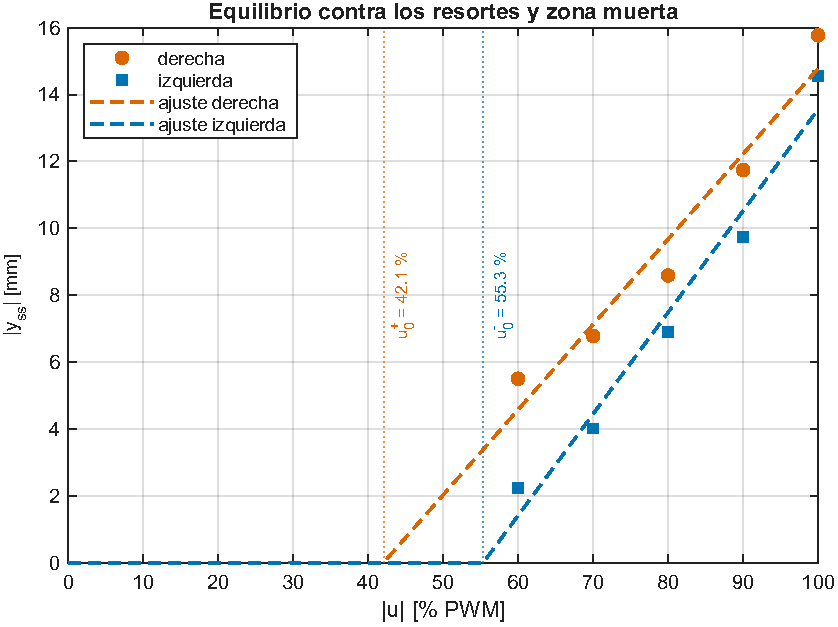
\includegraphics[width=0.85\linewidth]{equilibrio_pwm.pdf}
  \caption{Equilibrio contra los resortes vs. PWM: zona muerta por lado.}
  \label{fig:eq}
\end{figure}

\begin{figure*}[!t]
  \centering
  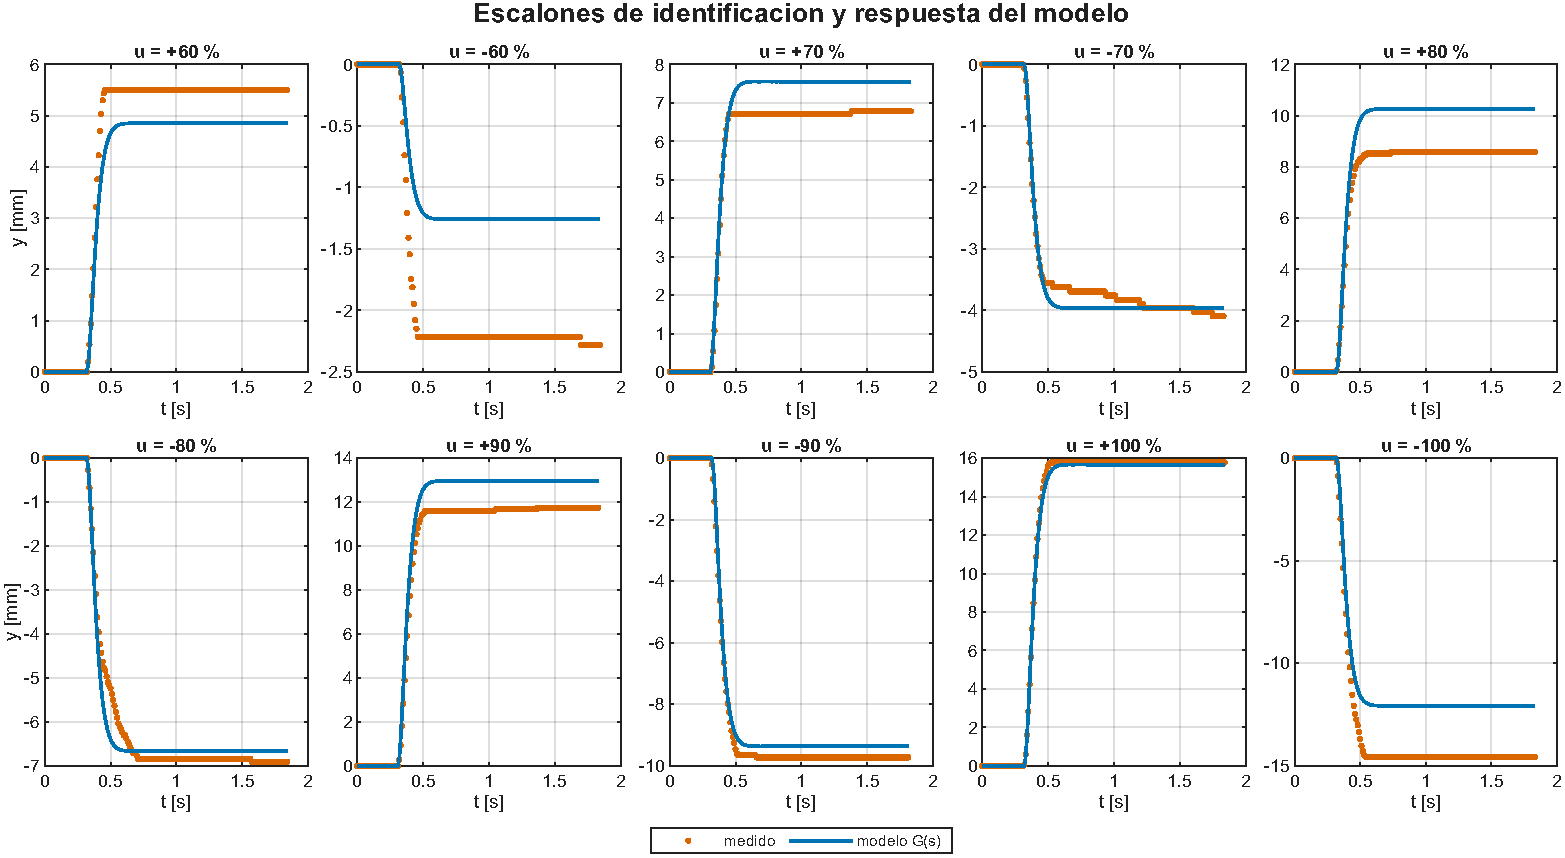
\includegraphics[width=0.92\textwidth]{ajuste_escalones.pdf}
  \caption{Escalones medidos (puntos) y respuesta del modelo identificado (línea).}
  \label{fig:ajuste}
\end{figure*}

\subsection{Tiempo de muestreo}
\begin{table}[!htb]
\centering
\caption{Criterios para el tiempo de muestreo}
\label{tab:T}
\begin{tabular}{lc}
\toprule
Criterio & Rango de $T$ [s]\\
\midrule
Landau, $0.25 \le \omega_n T \le 1.5$ & $0.0100$ -- $0.0601$\\
Lazo cerrado, $t_s/20$ -- $t_s/10$ & $0.0085$ -- $0.0171$\\
Lazo abierto, $t_s/80$ -- $t_s/40$ & $0.0021$ -- $0.0043$\\
\bottomrule
\end{tabular}
\end{table}
Se eligió $T = 10$~ms ($\omega_nT = 0.25$, $t_s/T = 17$), que cumple el
criterio de lazo cerrado y el límite inferior de Landau (Tabla~\ref{tab:T}).
El criterio de lazo abierto daría 2--4~ms, pero a la velocidad máxima medida
($\approx135$~mm/s) la masa recorre menos de 8 cuentas en ese tiempo y la
velocidad estimada sería ruidosa.

\subsection{Discretización de la planta}
La planta se discretiza con retenedor de orden cero (ZOH), que es lo que hace
el PWM: mantiene $u(k)$ constante durante todo el periodo. Por definición
\cite{ogata1995},
\begin{equation}
  G(z) = (1 - z^{-1})\,\mathcal{Z}\!\left\{\frac{G(s)}{s}\right\}.
  \label{eq:zoh}
\end{equation}

\textit{Paso 1: polos de la planta.} Las raíces de $s^2 + 46.87s + 622.9$ son
\begin{align*}
  s &= -\frac{46.87}{2} \pm j\sqrt{622.9 - \left(\frac{46.87}{2}\right)^{2}}\\
    &= -a \pm j\omega = -23.435 \pm j8.585,
\end{align*}
por lo que el denominador se escribe $(s+a)^2 + \omega^2$ y
$G(s) = b_0/[(s+a)^2+\omega^2]$, con $b_0 = 168.4$ y $a^2+\omega^2 = a_0 = 622.9$.

\textit{Paso 2: fracciones parciales.} Como los polos son complejos, se usa la
forma que aparece en la tabla de transformadas:
\begin{equation}
  \frac{G(s)}{s} = \frac{A}{s} + \frac{B(s+a) + C\omega}{(s+a)^2+\omega^2}.
  \label{eq:fp}
\end{equation}
Al multiplicar por $s[(s+a)^2+\omega^2]$ queda
\begin{align*}
  b_0 = A\left[(s+a)^2+\omega^2\right] + B(s+a)s + C\omega s,
\end{align*}
e igualando los coeficientes de cada potencia de $s$:
\begin{align*}
  s^0:&\quad b_0 = A\,(a^2+\omega^2) = A\,a_0,\\
  s^2:&\quad 0 = A + B,\\
  s^1:&\quad 0 = 2aA + aB + C\omega,
\end{align*}
de donde
\begin{align*}
  A &= b_0/a_0 = 168.4/622.9 = 0.270348,\\
  B &= -A = -0.270348,\\
  C &= -aA/\omega = -0.737994.
\end{align*}

\textit{Paso 3: transformada Z de cada término.} Para no arrastrar
exponenciales se definen
\begin{equation}
  \rho = e^{-aT},\qquad c = \cos\omega T,\qquad \sigma = \sin\omega T,
  \label{eq:sym}
\end{equation}
\begin{equation}
  D(z) = 1 - 2\rho c\,z^{-1} + \rho^2 z^{-2},
  \label{eq:Dz}
\end{equation}
y de la tabla \cite{ogata1995}:
\begin{align*}
  \mathcal{Z}\Big\{\frac{1}{s}\Big\} &= \frac{1}{1-z^{-1}},\\
  \mathcal{Z}\Big\{\frac{s+a}{(s+a)^2+\omega^2}\Big\} &= \frac{1-\rho c\,z^{-1}}{D(z)},\\
  \mathcal{Z}\Big\{\frac{\omega}{(s+a)^2+\omega^2}\Big\} &= \frac{\rho\sigma\,z^{-1}}{D(z)}.
\end{align*}
Con $T = 0.01$~s, $aT = 0.23435$ y $\omega T = 0.085849$~rad:
\begin{align*}
  \rho &= 0.791085, & \rho c &= 0.788171,\\
  c &= 0.996317, & \rho\sigma &= 0.067831,\\
  \sigma &= 0.085744, & \rho^2 &= 0.625815.
\end{align*}

\textit{Paso 4: aplicar (\ref{eq:zoh}).} Se transforma (\ref{eq:fp}) término
a término con los símbolos de (\ref{eq:sym}) y el denominador (\ref{eq:Dz}).
Al multiplicar por $(1-z^{-1})$, el primer término se reduce a $A$:
\begin{align*}
  G(z) = A + (1-z^{-1})\,\frac{B + (C\rho\sigma - B\rho c)\,z^{-1}}{D(z)}.
\end{align*}
Llamando $E = C\rho\sigma - B\rho c$ y sumando sobre el denominador común, el
numerador es
\begin{align*}
  N(z) &= A\,D(z) + (1-z^{-1})(B + E z^{-1})\\
       &= (A+B) + (E - B - 2A\rho c)\,z^{-1}\\
       &\quad + (A\rho^2 - E)\,z^{-2}.
\end{align*}
El término independiente se anula porque $B = -A$, y con $E = C\rho\sigma +
A\rho c$ la planta discreta toma la forma general
\begin{equation}
  G(z) = \frac{b_1z^{-1} + b_2z^{-2}}{1 + d_1z^{-1} + d_2z^{-2}}
  \label{eq:Gzgen}
\end{equation}
con
\begin{align*}
  b_1 &= A(1-\rho c) + C\rho\sigma, & d_1 &= -2\rho c,\\
  b_2 &= A(\rho^2-\rho c) - C\rho\sigma, & d_2 &= \rho^2.
\end{align*}
Sustituyendo los valores de los pasos 2 y 3:
\begin{align*}
  b_1 &= 0.270348(1 - 0.788171)\\
      &\quad - 0.737994(0.067831)\\
      &= 0.057267 - 0.050059 = 0.007209,\\[3pt]
  b_2 &= 0.270348(0.625815 - 0.788171)\\
      &\quad + 0.050059\\
      &= -0.043893 + 0.050059 = 0.006166,\\[3pt]
  d_1 &= -2(0.788171) = -1.576343,\qquad d_2 = 0.625815,
\end{align*}
es decir,
\begin{equation}
  G(z) = \frac{0.007209\,z^{-1} + 0.006166\,z^{-2}}{1 - 1.576343\,z^{-1} + 0.625815\,z^{-2}}.
  \label{eq:Gz}
\end{equation}

\textit{Paso 5: verificación.} El resultado coincide con
\texttt{c2d(Gs,0.01,'zoh')} y cumple tres comprobaciones:
\begin{itemize}
  \item Ganancia DC: $G(1) = (b_1+b_2)/(1+d_1+d_2) = 0.013375/0.049472
        = 0.2703$, igual a $K = b_0/a_0$.
  \item Polos: $z = \rho\,e^{\pm j\omega T} = 0.788 \pm j0.068$, con
        $|z| = \rho = 0.791$; son $e^{sT}$ de los polos continuos.
  \item Cero: $z = -b_2/b_1 = -0.855$, el cero que agrega el muestreo con ZOH.
\end{itemize}
La Fig.~\ref{fig:zoh} muestra que la respuesta de (\ref{eq:Gz}) pasa por la de
$G(s)$ en cada instante de muestreo.

\begin{figure}[!htb]
  \centering
  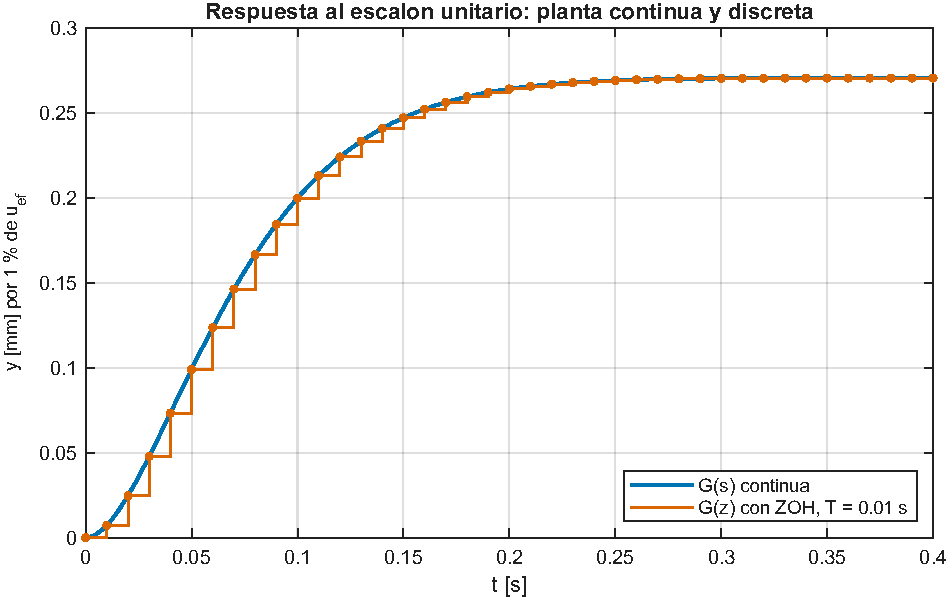
\includegraphics[width=\linewidth]{escalon_continuo_discreto.pdf}
  \caption{Escalón unitario de $G(s)$ y de $G(z)$ con ZOH.}
  \label{fig:zoh}
\end{figure}

\subsection{Especificaciones}
Para comparar en igualdad de condiciones, ambos controladores usan el mismo
polinomio deseado. Se pidió $\zeta_d = 1$ (sin sobrepico) y $t_{s,d} = 0.3$~s
($\approx1.75$ veces el $t_s$ de lazo abierto, para no llevar el actuador a
saturación permanente):
\begin{align*}
  \omega_{n,d} &= \frac{4}{\zeta_d\,t_{s,d}} = \frac{4}{(1)(0.3)} = 13.333~\text{rad/s},\\
  p_3 &= 5\,\zeta_d\,\omega_{n,d} = 66.667~\text{rad/s}.
\end{align*}
En la práctica 3 se usó $p_3 = 10\zeta\omega_n$, pero aquí daría $p_3T = 1.33$ y
Euler deformaría el lazo (28.6~\% de sobrepico en la simulación lineal); con
$5\zeta\omega_n$, $p_3T = 0.67$ y la respuesta discreta conserva la continua.

\subsection{Controlador PID continuo--discreto}
\textit{Paso 1: ecuación característica.} Con
$C(s) = K_p + K_i/s + K_ds = (K_ds^2 + K_ps + K_i)/s$, el lazo cerrado cumple
$1 + C(s)G(s) = 0$:
\begin{align*}
  1 + \frac{K_ds^2 + K_ps + K_i}{s}\cdot\frac{b_0}{s^2 + a_1s + a_0} = 0.
\end{align*}
Al multiplicar por $s(s^2+a_1s+a_0)$ y agrupar por potencias de $s$:
\begin{equation}
  s^3 + (a_1 + b_0K_d)s^2 + (a_0 + b_0K_p)s + b_0K_i = 0.
  \label{eq:carS}
\end{equation}

\textit{Paso 2: polinomio deseado.}
\begin{align*}
  P_d(s) &= (s^2 + 2\zeta_d\omega_{n,d}s + \omega_{n,d}^2)(s + p_3)\\
         &= (s^2 + 26.667s + 177.78)(s + 66.667),
\end{align*}
cuyos coeficientes son
\begin{align*}
  s^2:&\quad 26.667 + 66.667 = 93.333,\\
  s^1:&\quad 177.78 + (26.667)(66.667) = 1955.56,\\
  s^0:&\quad (177.78)(66.667) = 11851.85.
\end{align*}

\textit{Paso 3: igualar.} Comparando (\ref{eq:carS}) con $P_d(s)$ término a
término, cada ganancia queda despejada de una sola ecuación:
\begin{align*}
  K_d &= \frac{93.333 - 46.87}{168.4} = 0.2759,\\
  K_p &= \frac{1955.56 - 622.9}{168.4} = 7.9136,\\
  K_i &= \frac{11851.85}{168.4} = 70.3792.
\end{align*}

\textit{Paso 4: Euler hacia atrás.} Se sustituye $s \approx (1-z^{-1})/T$ en
cada término del PID:
\begin{align*}
  K_p &\;\rightarrow\; K_p,\\
  \frac{K_i}{s} &\;\rightarrow\; \frac{K_iT}{1-z^{-1}},\\
  K_d\,s &\;\rightarrow\; \frac{K_d}{T}\,(1-z^{-1}).
\end{align*}
Sobre el denominador común $1-z^{-1}$:
\begin{align*}
  C_1(z) = \frac{K_p(1-z^{-1}) + K_iT + \frac{K_d}{T}(1-z^{-1})^2}{1-z^{-1}}.
\end{align*}
Desarrollando $(1-z^{-1})^2 = 1 - 2z^{-1} + z^{-2}$ y agrupando,
\begin{equation}
  C_1(z) = \frac{q_0 + q_1z^{-1} + q_2z^{-2}}{1 - z^{-1}}
  \label{eq:C1}
\end{equation}
con
\begin{align*}
  q_0 &= K_p + K_iT + K_d/T,\\
  q_1 &= -K_p - 2K_d/T,\\
  q_2 &= K_d/T.
\end{align*}
Con $K_d/T = 27.5911$ y $K_iT = 0.7038$:
\begin{align*}
  q_0 &= 7.9136 + 0.7038 + 27.5911 = 36.2085,\\
  q_1 &= -7.9136 - 2(27.5911) = -63.0957,\\
  q_2 &= 27.5911.
\end{align*}

\textit{Paso 5: ecuación en diferencias.} De (\ref{eq:C1}),
$U(z)(1-z^{-1}) = (q_0 + q_1z^{-1} + q_2z^{-2})E(z)$, y al pasar al dominio
del tiempo:
\begin{equation}
  u(k) = u(k-1) + q_0e(k) + q_1e(k-1) + q_2e(k-2).
  \label{eq:ukcd}
\end{equation}
Los valores numéricos están en la Tabla~\ref{tab:coef}.

\subsection{Controlador discreto--discreto}
\textit{Paso 1: estructura.} Sobre la planta (\ref{eq:Gzgen}), con
$B(z) = b_1z^{-1} + b_2z^{-2}$ y $A(z) = 1 + d_1z^{-1} + d_2z^{-2}$, se
propone
\begin{equation}
  C_2(z) = \frac{Q(z)}{(1-z^{-1})(1+s_0z^{-1})},
  \label{eq:C2}
\end{equation}
con $Q(z) = q_0 + q_1z^{-1} + q_2z^{-2}$. El factor $(1-z^{-1})$ es un
integrador, que asegura $e_{ss} = 0$. De $1 + C_2(z)G(z) = 0$:
\begin{equation}
  A(z)(1-z^{-1})(1+s_0z^{-1}) + B(z)Q(z) = 0.
  \label{eq:carZ}
\end{equation}
Es un polinomio de cuarto orden en $z^{-1}$ con cuatro incógnitas
($q_0$, $q_1$, $q_2$, $s_0$), así que se pueden fijar los cuatro polos.

\textit{Paso 2: polos deseados.} Cada polo continuo se lleva al plano $z$ con
$z = e^{sT}$. Con $\zeta_d = 1$ el par dominante es un polo doble en
$s = -\omega_{n,d}$, y el tercer polo se duplica para completar el orden:
\begin{align*}
  z_{1,2} &= e^{-\omega_{n,d}T} = e^{-0.13333} = 0.875173,\\
  z_{3,4} &= \alpha = e^{-p_3T} = e^{-0.66667} = 0.513417.
\end{align*}
El factor dominante $1 + P_1z^{-1} + P_2z^{-2}$ tiene
\begin{align*}
  P_1 &= -2e^{-\zeta\omega_nT}\cos\!\left(\omega_nT\sqrt{1-\zeta^2}\right)\\
      &= -2(0.875173)(1) = -1.750347,\\[2pt]
  P_2 &= e^{-2\zeta\omega_nT} = 0.875173^2 = 0.765928,
\end{align*}
y el factor rápido es
$(1-\alpha z^{-1})^2 = 1 - 1.026834\,z^{-1} + 0.263597\,z^{-2}$. Su producto es
\begin{equation}
  P_d(z) = 1 + \delta_1z^{-1} + \delta_2z^{-2} + \delta_3z^{-3} + \delta_4z^{-4}
  \label{eq:Pdz}
\end{equation}
con
\begin{align*}
  \delta_1 &= P_1 - 2\alpha = -2.777181,\\
  \delta_2 &= P_2 - 2\alpha P_1 + \alpha^2 = 2.826841,\\
  \delta_3 &= \alpha^2P_1 - 2\alpha P_2 = -1.247868,\\
  \delta_4 &= \alpha^2P_2 = 0.201897.
\end{align*}

\textit{Paso 3: desarrollar (\ref{eq:carZ}).} Primero se multiplica la planta
por el integrador:
\begin{align*}
  A(z)(1-z^{-1}) = 1 + h_1z^{-1} + h_2z^{-2} + h_3z^{-3},
\end{align*}
\begin{align*}
  h_1 &= d_1 - 1 = -2.576343,\\
  h_2 &= d_2 - d_1 = 2.202158,\\
  h_3 &= -d_2 = -0.625815.
\end{align*}
Al multiplicar por $(1+s_0z^{-1})$ y sumar $B(z)Q(z)$, el coeficiente de cada
potencia es
\begin{align*}
  z^{-1}:&\quad h_1 + s_0 + b_1q_0,\\
  z^{-2}:&\quad h_2 + h_1s_0 + b_2q_0 + b_1q_1,\\
  z^{-3}:&\quad h_3 + h_2s_0 + b_2q_1 + b_1q_2,\\
  z^{-4}:&\quad h_3s_0 + b_2q_2.
\end{align*}

\textit{Paso 4: igualar con (\ref{eq:Pdz}).} Cada coeficiente debe ser igual a
$\delta_i$, lo que da un sistema lineal en las incógnitas:
\begin{align*}
  b_1q_0 + s_0 &= \delta_1 - h_1,\\
  b_2q_0 + b_1q_1 + h_1s_0 &= \delta_2 - h_2,\\
  b_2q_1 + b_1q_2 + h_2s_0 &= \delta_3 - h_3,\\
  b_2q_2 + h_3s_0 &= \delta_4.
\end{align*}
En forma matricial, con los valores numéricos,
\begin{align*}
\resizebox{0.92\linewidth}{!}{$
\begin{bmatrix}
 0.007209 & 0 & 0 & 1\\
 0.006166 & 0.007209 & 0 & -2.576343\\
 0 & 0.006166 & 0.007209 & 2.202158\\
 0 & 0 & 0.006166 & -0.625815
\end{bmatrix}
\begin{bmatrix} q_0\\ q_1\\ q_2\\ s_0 \end{bmatrix}
=
\begin{bmatrix} -0.200838\\ 0.624683\\ -0.622053\\ 0.201897 \end{bmatrix}
$}
\end{align*}
cuya solución es
\begin{align*}
  q_0 &= 8.5234, & q_1 &= -14.3710,\\
  q_2 &= 6.1235, & s_0 &= -0.262282.
\end{align*}

\textit{Paso 5: ecuación en diferencias.} De (\ref{eq:C2}),
$U(z)(1-z^{-1})(1+s_0z^{-1}) = Q(z)E(z)$. Como
$(1-z^{-1})(1+s_0z^{-1}) = 1 - (1-s_0)z^{-1} - s_0z^{-2}$,
\begin{multline}
  u(k) = (1-s_0)\,u(k-1) + s_0\,u(k-2)\\
  + q_0e(k) + q_1e(k-1) + q_2e(k-2).
  \label{eq:ukdd}
\end{multline}
Con $s_0 = 0$ esta expresión se reduce a (\ref{eq:ukcd}), por eso el
firmware usa una sola rutina para los dos controladores y solo cambia los
coeficientes de la Tabla~\ref{tab:coef}.

\textit{Verificación.} Las raíces de (\ref{eq:carZ}) con estos coeficientes son
$z = 0.875$ (doble) y $z = 0.513$ (doble), exactamente las deseadas. En cambio,
el lazo con $C_1(z)$ queda con polos en $0.890$, $0.872$ y
$0.277 \pm j0.378$: Euler conserva aproximadamente el par dominante, pero
mueve el polo rápido.

\begin{table}[!htb]
\centering
\caption{Coeficientes de los dos controladores}
\label{tab:coef}
\setlength{\tabcolsep}{5pt}
\resizebox{\columnwidth}{!}{%
\begin{tabular}{lcc}
\toprule
 & Continuo--discreto & Discreto--discreto\\
 & ec.~(\ref{eq:ukcd}) & ec.~(\ref{eq:ukdd})\\
\midrule
$K_p$, $K_i$, $K_d$ & 7.914, 70.38, 0.276 & --\\
$q_0$ & 36.2085 & 8.5234\\
$q_1$ & $-63.0957$ & $-14.3710$\\
$q_2$ & 27.5911 & 6.1235\\
$s_0$ & 0 & $-0.262282$\\
\midrule
Polos lentos & 0.890, 0.872 & 0.875 (doble)\\
Polos rápidos & $0.277 \pm j0.378$ & 0.513 (doble)\\
\bottomrule
\end{tabular}}
\end{table}

\FloatBarrier
\subsection{Simulación en MATLAB/Simulink}

\subsubsection{Estructura del modelo}
El modelo \texttt{lab5\_control.slx} se construyó con un script de MATLAB
(\texttt{crear\_modelo.m}); los parámetros de la planta y los coeficientes de
los controladores se cargan desde \texttt{parametros.m} al iniciar cada
simulación, de modo que el modelo usa exactamente los valores calculados en el
diseño. El nivel superior (Fig.~\ref{fig:sl}) tiene:
\begin{itemize}
  \item \textbf{Referencia}: dos bloques \textit{Step} sumados, que dan
        $r = +5$~mm en $t = 0.1$~s y $r = -5$~mm en $t = 1.6$~s, para probar
        ambos sentidos de movimiento.
  \item \textbf{Tres subsistemas}, uno por lazo, alimentados con la misma
        referencia: PID continuo, continuo--discreto y discreto--discreto.
        Cada uno entrega $y$, $u$ y $e$.
  \item \textbf{ISE}: para cada lazo, $e$ pasa por un bloque $e^2$ y un
        integrador, cuyo valor final se muestra en un \textit{Display}.
  \item \textbf{Scopes} de posición, control y error, y bloques
        \textit{To Workspace} que guardan todas las señales para graficarlas
        y calcular las métricas.
\end{itemize}
Se usó el solver de paso fijo \texttt{ode4} con paso de $10^{-4}$~s, cien
veces menor que $T$, para que la planta continua se integre con precisión
entre muestras.

\begin{figure*}[!t]
  \centering
  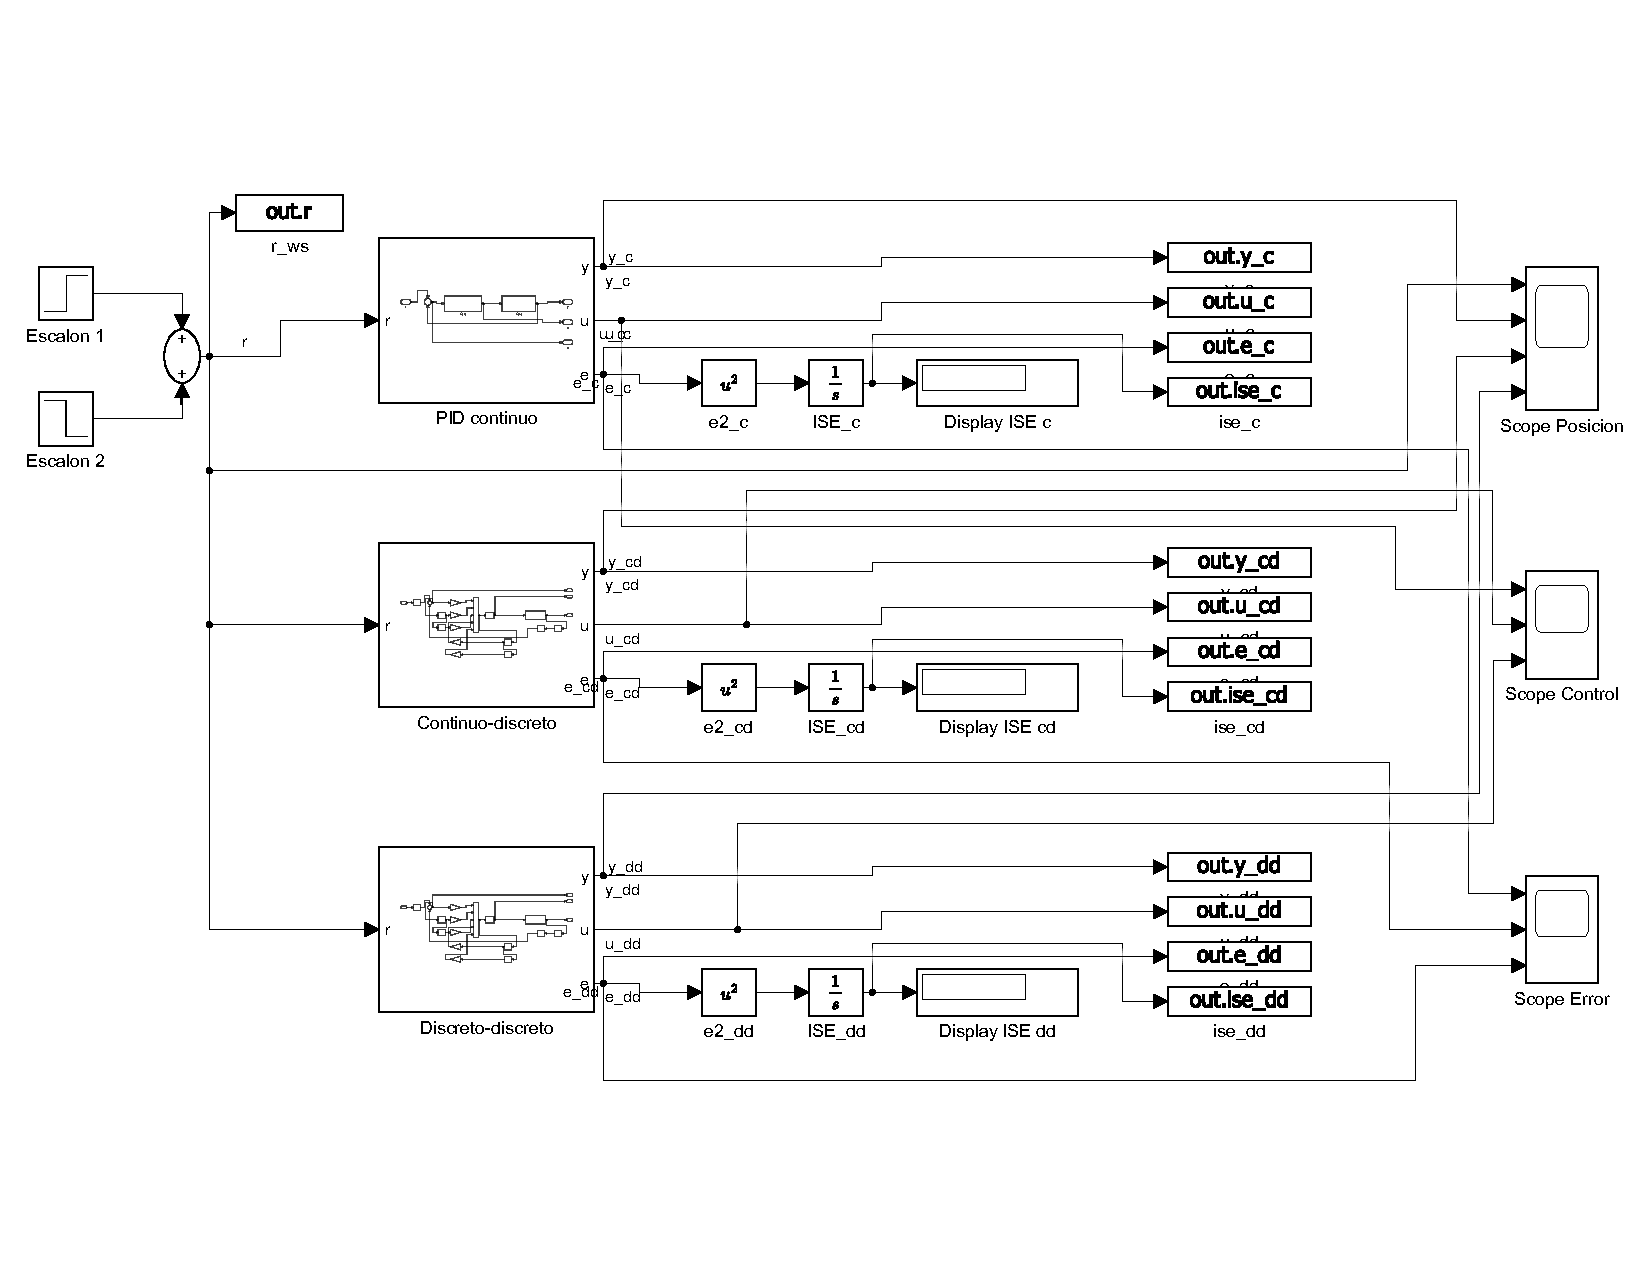
\includegraphics[width=0.8\textwidth]{simulink_modelo.pdf}
  \caption{Nivel superior del modelo de Simulink: referencia, los tres lazos,
  cálculo del ISE, scopes y registro de señales.}
  \label{fig:sl}
\end{figure*}

\begin{figure*}[!t]
  \centering
  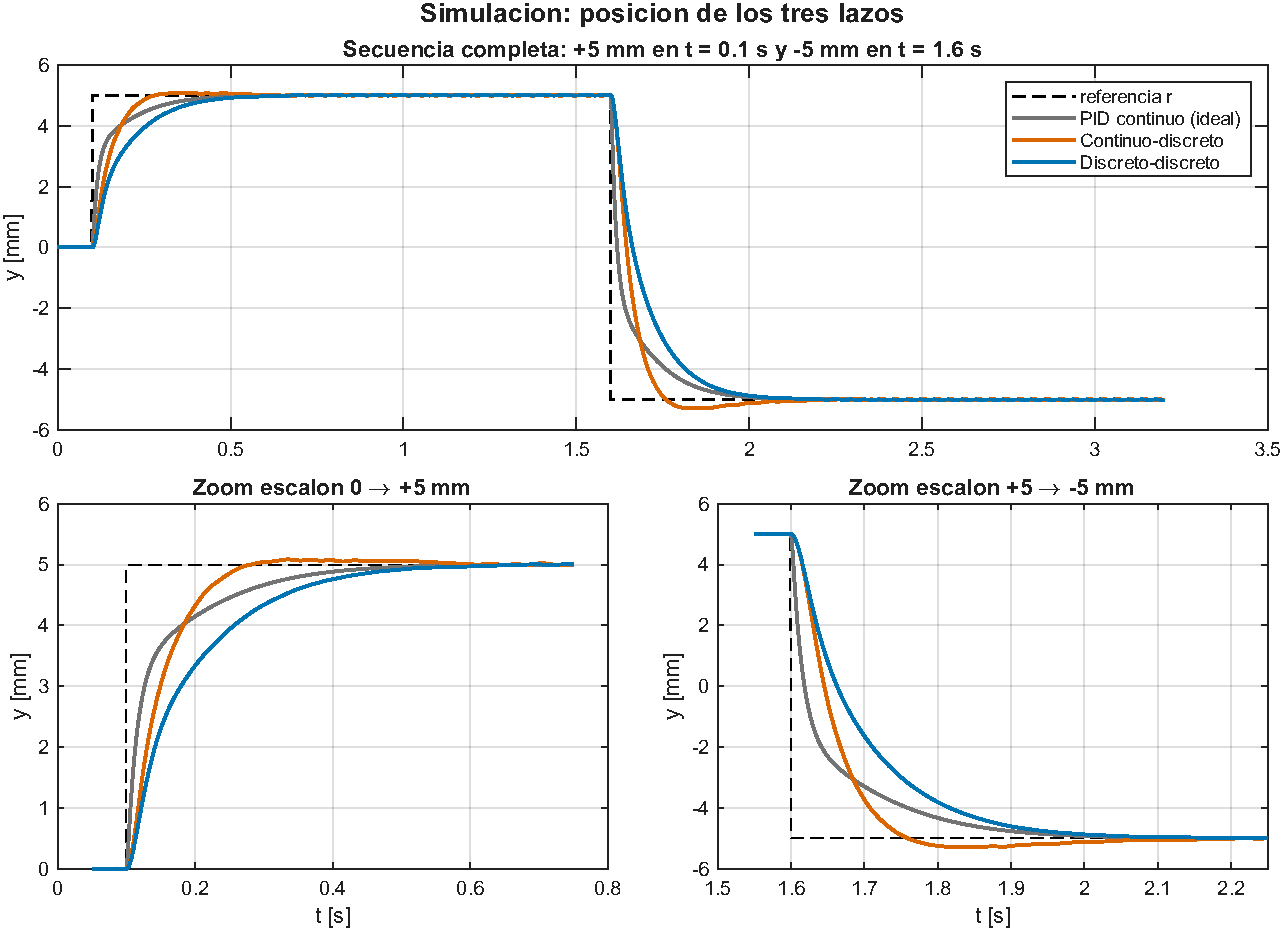
\includegraphics[width=0.85\textwidth]{sim_posicion.pdf}
  \caption{Posición simulada de los tres lazos: secuencia completa (arriba) y
  acercamiento a cada escalón (abajo).}
  \label{fig:simpos}
\end{figure*}

\subsubsection{Lazo continuo de referencia}
El subsistema \textit{PID continuo} (Fig.~\ref{fig:slpid}) cierra el lazo con
$C(s) = (K_ds^2 + K_ps + K_i)/s$ y la planta $G(s)$ de (\ref{eq:Gs}). Para que
el bloque sea propio, el derivativo lleva un filtro de primer orden con polo
en 1000~rad/s, muy por encima de la dinámica del lazo. No tiene saturación:
representa el diseño ideal que se quiere aproximar en discreto.

\begin{figure}[H]
  \centering
  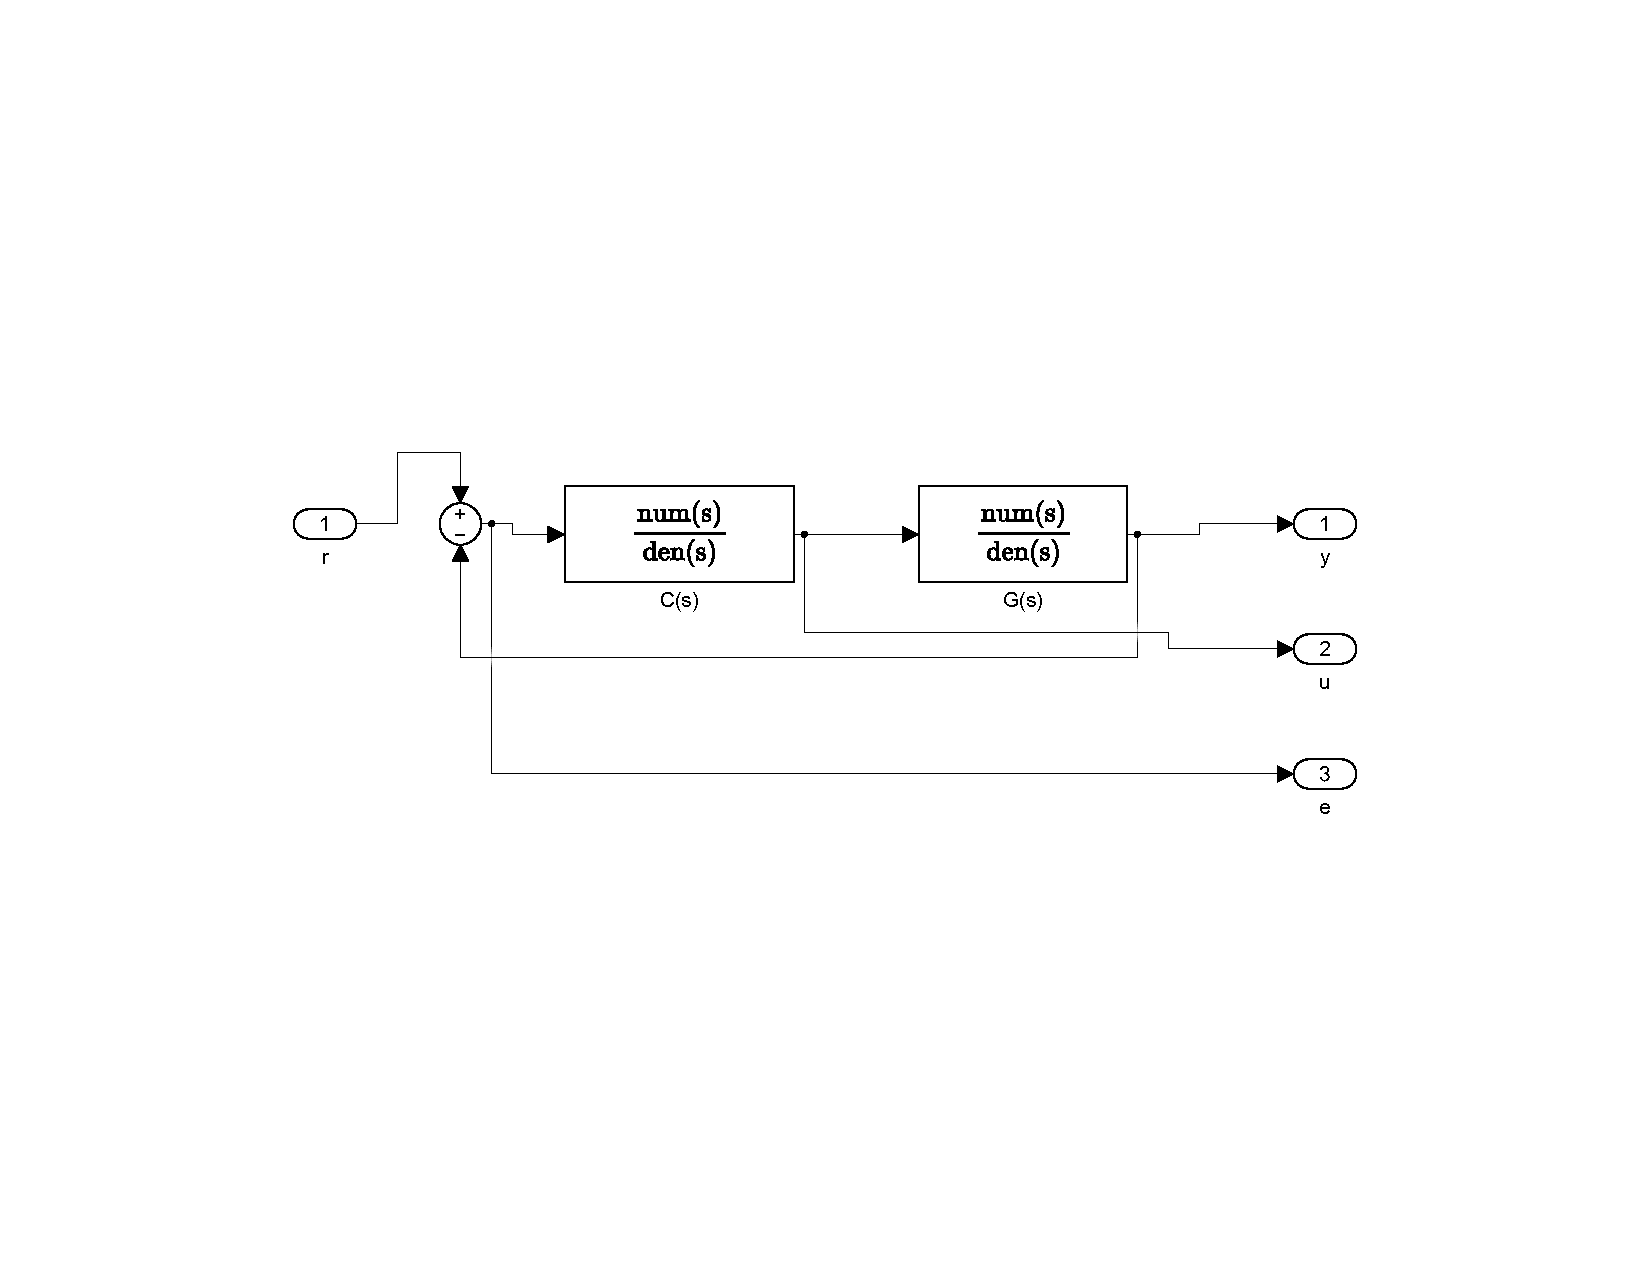
\includegraphics[width=\linewidth]{simulink_pid_continuo.pdf}
  \caption{Subsistema del PID continuo ideal.}
  \label{fig:slpid}
\end{figure}

\subsubsection{Lazos discretos}
Los dos subsistemas discretos (Fig.~\ref{fig:sldisc}) tienen
la misma estructura y solo cambian los coeficientes; reproducen, bloque por
bloque, lo que hace el microcontrolador:
\begin{enumerate}
  \item \textbf{Muestreo}: un ZOH de periodo $T$ muestrea la referencia y otro
        la salida de la planta.
  \item \textbf{Sensor}: un cuantizador con paso de $0.0671$~mm convierte la
        posición en cuentas del encoder.
  \item \textbf{Ecuación en diferencias}: el error $e(k)$ y sus retardos
        $e(k-1)$ y $e(k-2)$ (bloques $z^{-1}$) se multiplican por $q_0$, $q_1$
        y $q_2$; los retardos $u(k-1)$ y $u(k-2)$ se multiplican por $1-s_0$ y
        $s_0$, y todo se suma. Para el continuo--discreto $s_0 = 0$.
  \item \textbf{Saturación}: limita $u_{ef}$ a $[-44.7,\ 57.9]~\%$, lo que
        queda del PWM después de la zona muerta.
  \item \textbf{Planta}: $G(s)$ continua, excitada por la señal escalonada que
        produce el ZOH implícito de la salida discreta.
\end{enumerate}
Los retardos de $u$ toman la señal \emph{antes} de la saturación. Con la señal
saturada en la memoria apareció un efecto indeseado: el salto del derivativo
satura la salida en $+57.9~\%$ y en la muestra siguiente el término
$q_1e(k-1) \approx -316~\%$ entra completo, de modo que la masa se movía
$1.1$~mm en sentido contrario antes de subir. Guardando $u$ sin saturar (con
una cota de $\pm300~\%$) el controlador se comporta como uno lineal seguido de
la saturación y el efecto desaparece. El firmware hace lo mismo.

\begin{figure}[H]
  \centering
  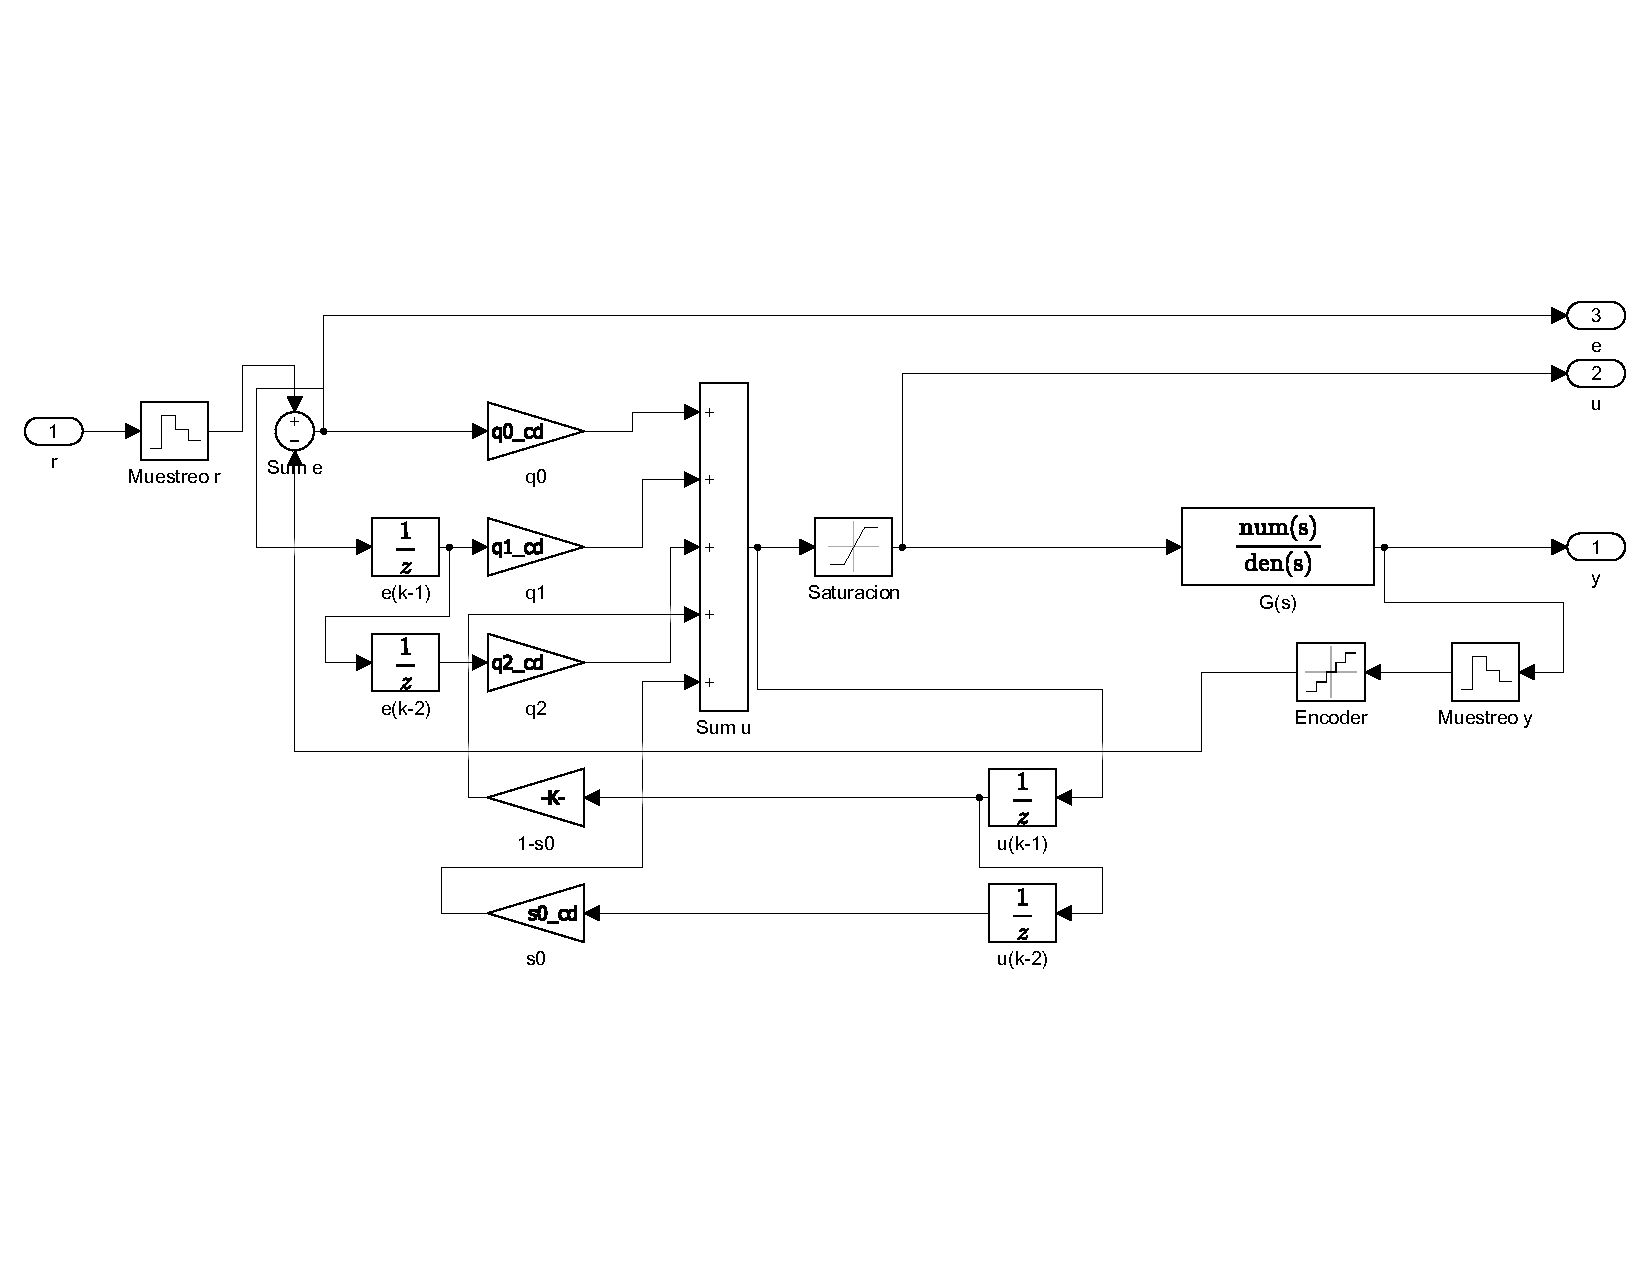
\includegraphics[width=\linewidth]{simulink_lazo_cd.pdf}\\
  {\footnotesize (a) Continuo--discreto: PID discretizado por Euler hacia atrás.}\\[4pt]
  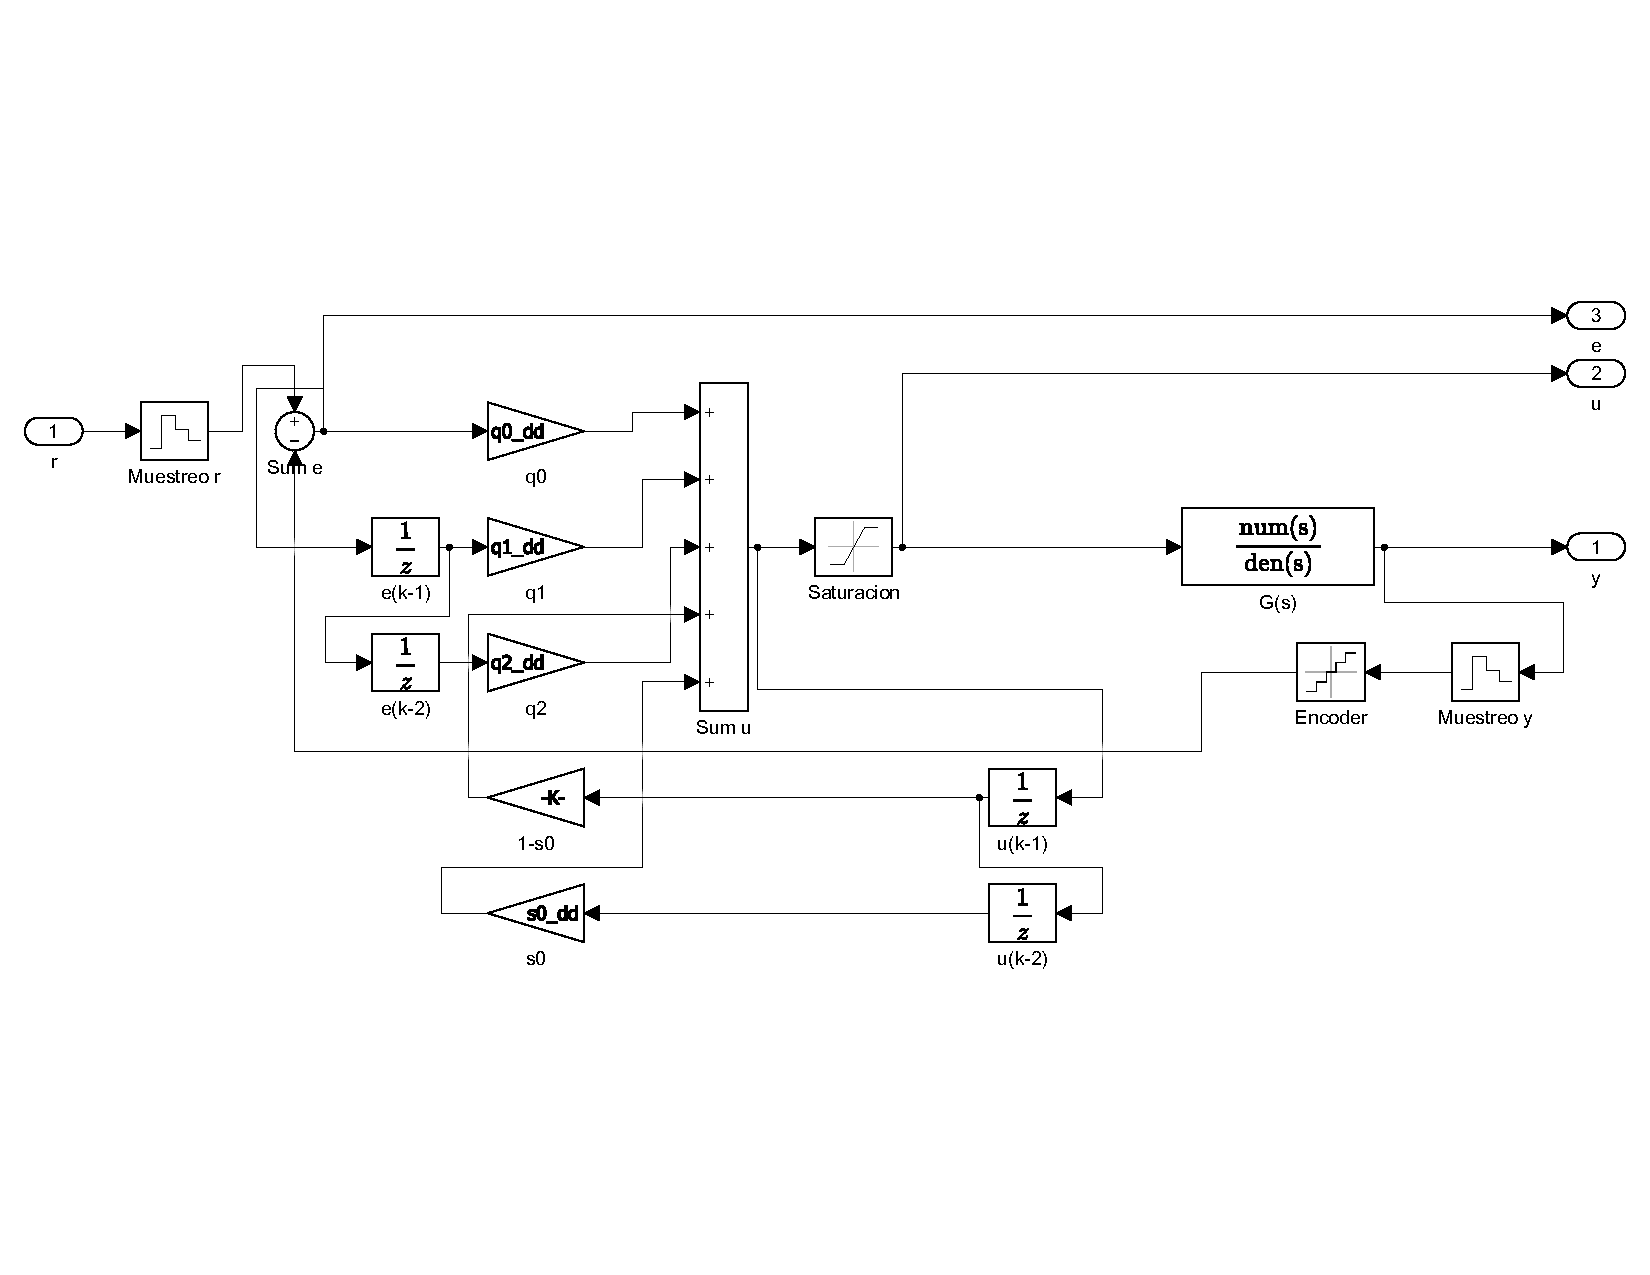
\includegraphics[width=\linewidth]{simulink_lazo_dd.pdf}\\
  {\footnotesize (b) Discreto--discreto: $q_0$, $q_1$, $q_2$ y $s_0$.}
  \caption{Subsistemas discretos de Simulink: muestreo, encoder, ecuación en
  diferencias, saturación y planta.}
  \label{fig:sldisc}
\end{figure}

\subsubsection{Resultados de la simulación}
La Fig.~\ref{fig:simpos} compara la posición de los tres lazos durante toda la
secuencia, con un acercamiento a cada escalón. La Fig.~\ref{fig:simcd}
muestra, para cada controlador discreto, la posición, la
acción de control con sus límites de saturación y el error. La
Fig.~\ref{fig:simu} compara la acción de control y la Fig.~\ref{fig:simise}
el ISE acumulado. Las métricas están en la Tabla~\ref{tab:sim}.

\begin{table}[H]
\centering
\caption{Resultados de simulación (ISE en mm$^2\cdot$s)}
\label{tab:sim}
\setlength{\tabcolsep}{4pt}
\resizebox{\columnwidth}{!}{%
\begin{tabular}{lcccccc}
\toprule
 & \multicolumn{3}{c}{$0\to5$ mm} & \multicolumn{3}{c}{$5\to-5$ mm}\\
\cmidrule(lr){2-4}\cmidrule(lr){5-7}
 & $t_s$ [s] & $M_p$ [\%] & ISE & $t_s$ [s] & $M_p$ [\%] & ISE\\
\midrule
PID ideal & 0.315 & 0.00 & 0.447 & 0.315 & 0.00 & 1.787\\
C--D      & 0.157 & 1.68 & 0.861 & 0.329 & 2.89 & 3.975\\
D--D      & 0.382 & 0.12 & 1.270 & 0.360 & 0.04 & 5.373\\
\bottomrule
\end{tabular}}
\end{table}

\begin{figure*}[!t]
  \centering
  \begin{minipage}[t]{0.49\textwidth}
    \centering
    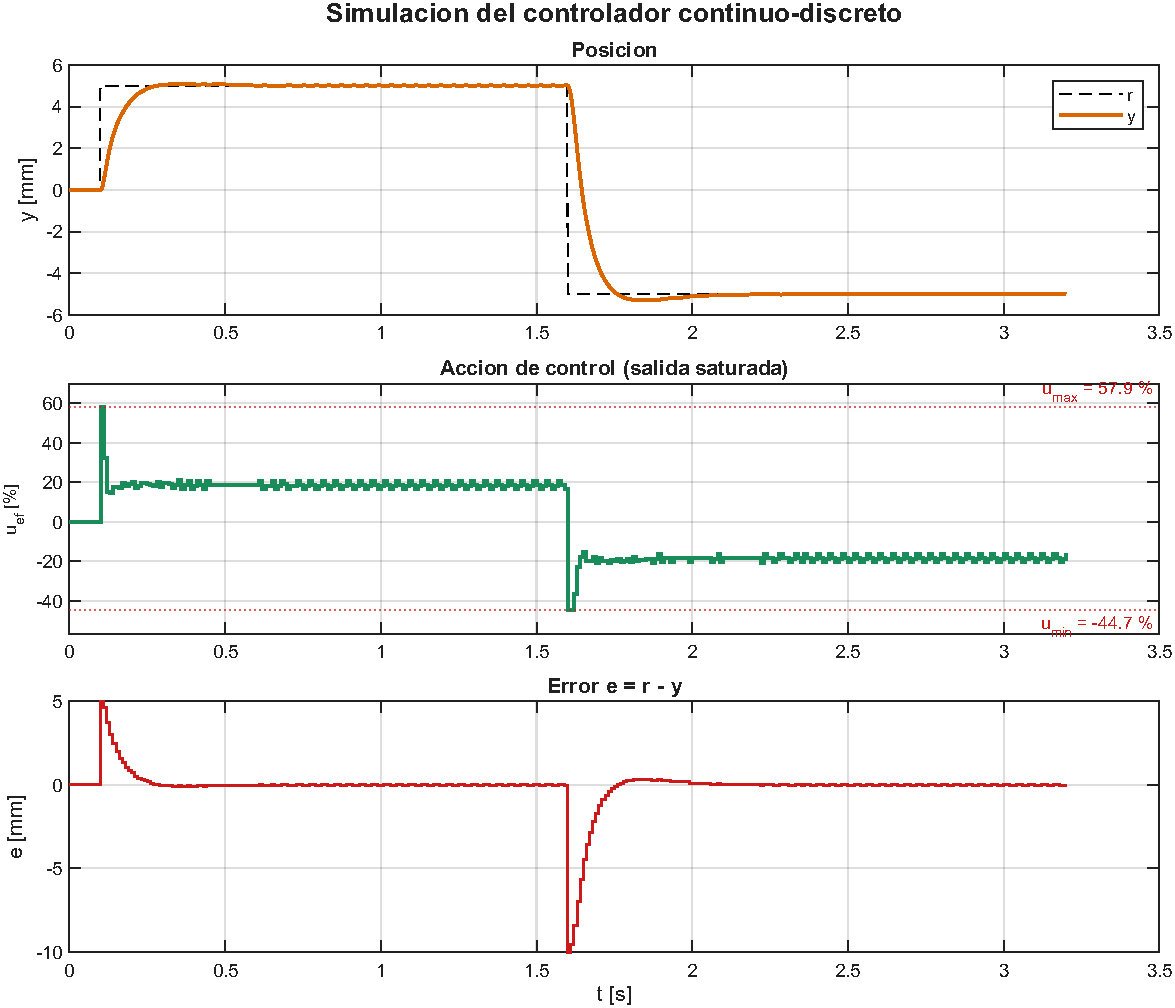
\includegraphics[width=\linewidth]{sim_cd.pdf}\\[2pt]
    {\footnotesize (a) Continuo--discreto.}
  \end{minipage}\hfill
  \begin{minipage}[t]{0.49\textwidth}
    \centering
    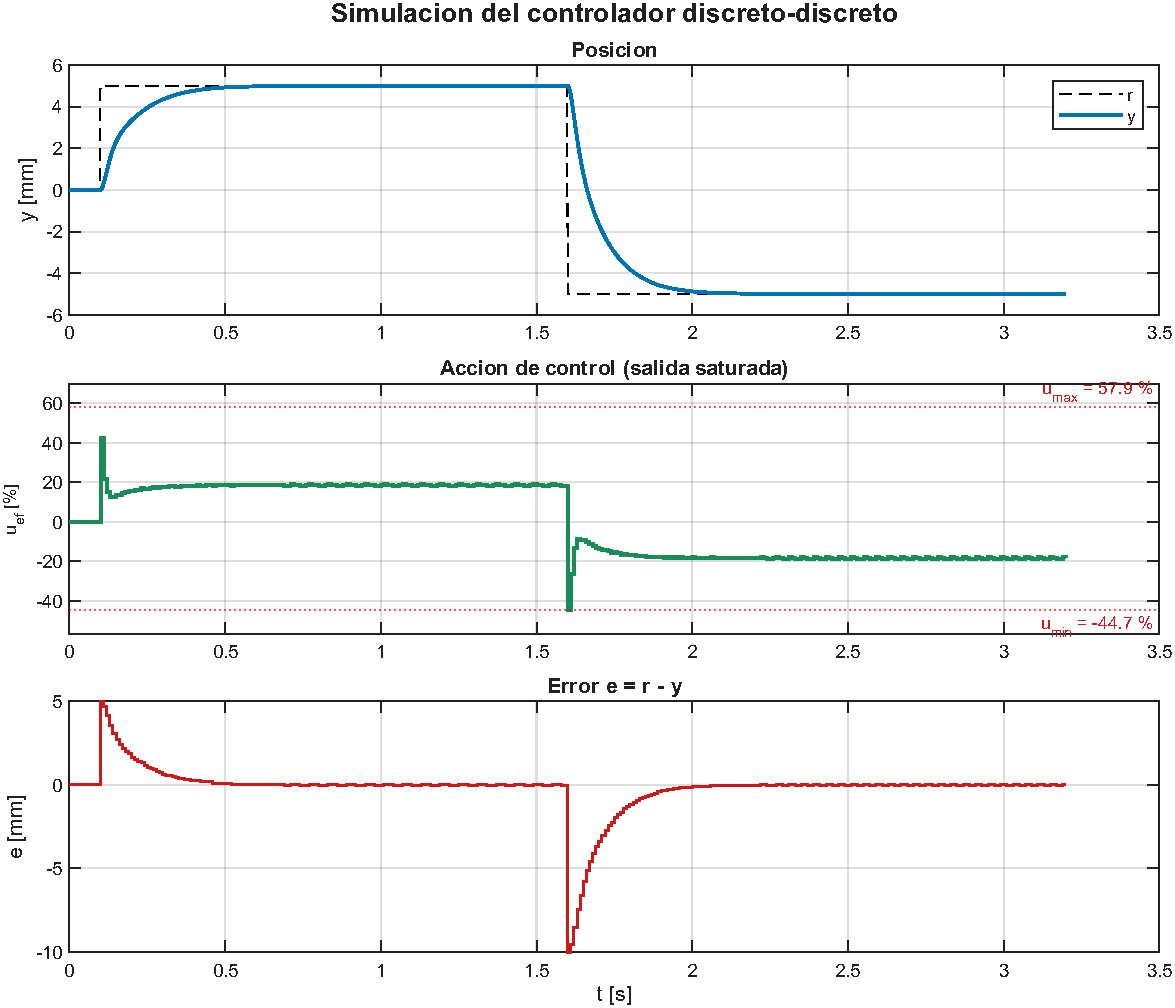
\includegraphics[width=\linewidth]{sim_dd.pdf}\\[2pt]
    {\footnotesize (b) Discreto--discreto.}
  \end{minipage}
  \caption{Simulación de cada controlador discreto: posición, acción de
  control con sus límites de saturación y error.}
  \label{fig:simcd}
\end{figure*}

\begin{figure}[H]
  \centering
  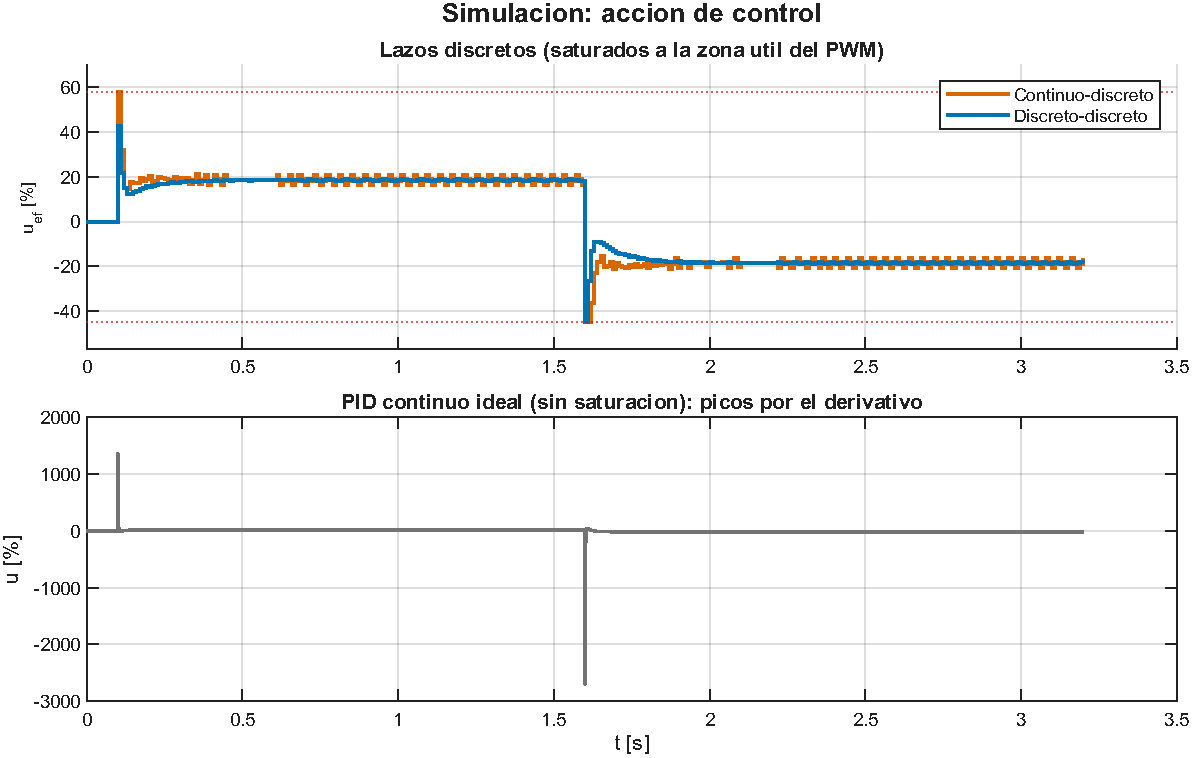
\includegraphics[width=\linewidth]{sim_control.pdf}
  \caption{Acción de control: lazos discretos saturados (arriba) y PID
  continuo ideal sin saturación (abajo).}
  \label{fig:simu}
\end{figure}

\begin{figure}[H]
  \centering
  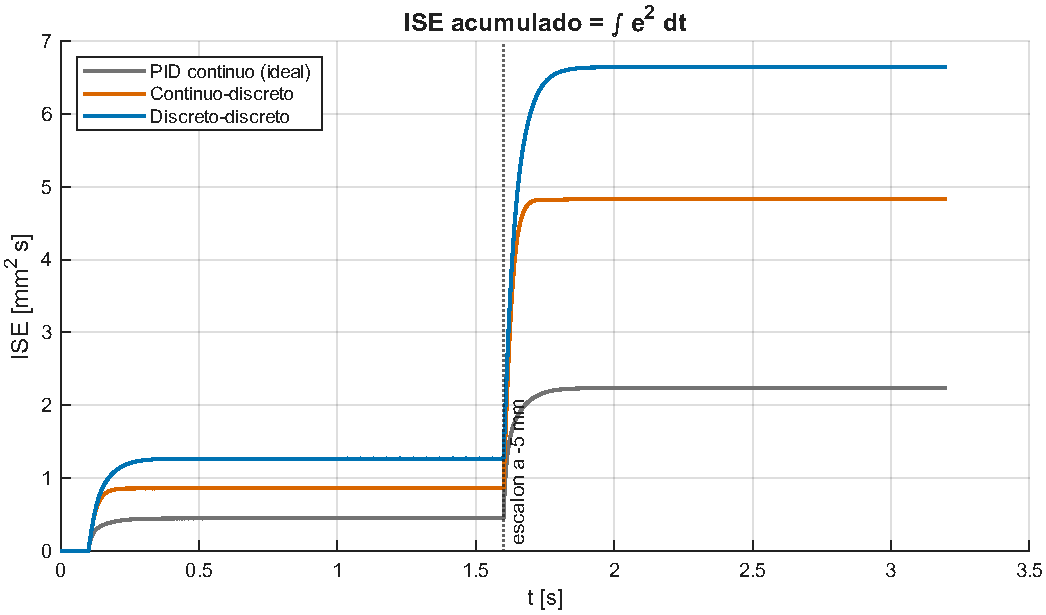
\includegraphics[width=\linewidth]{sim_ise.pdf}
  \caption{ISE acumulado de los tres lazos.}
  \label{fig:simise}
\end{figure}

De la simulación se observa que:
\begin{itemize}
  \item El PID continuo ideal es la referencia de diseño ($t_s = 0.315$~s, sin
        sobrepico), pero lo consigue con picos de control de hasta
        $1357~\%$ por el derivativo (Fig.~\ref{fig:simu}), imposibles en el
        actuador real.
  \item El continuo--discreto satura al inicio de cada escalón
        ($q_0 = 36.2$ multiplica el salto del error) y, al tener toda la
        autoridad disponible, es el más rápido de los lazos realistas
        ($t_s = 0.157$~s), con un sobrepico pequeño ($<3~\%$) y el menor ISE.
  \item El discreto--discreto, con ganancias unas cuatro veces menores, casi
        no satura, no tiene sobrepico y sus polos de lazo cerrado son
        exactamente los deseados; es más lento y acumula más ISE.
  \item Los tres llegan a $e_{ss} = 0$ por el integrador. La pequeña
        oscilación de $u_{ef}$ en estado estable (Fig.~\ref{fig:simcd}a) se debe
        a la cuantización del encoder: el error salta entre 0 y una cuenta.
\end{itemize}

\begin{figure*}[!t]
  \centering
  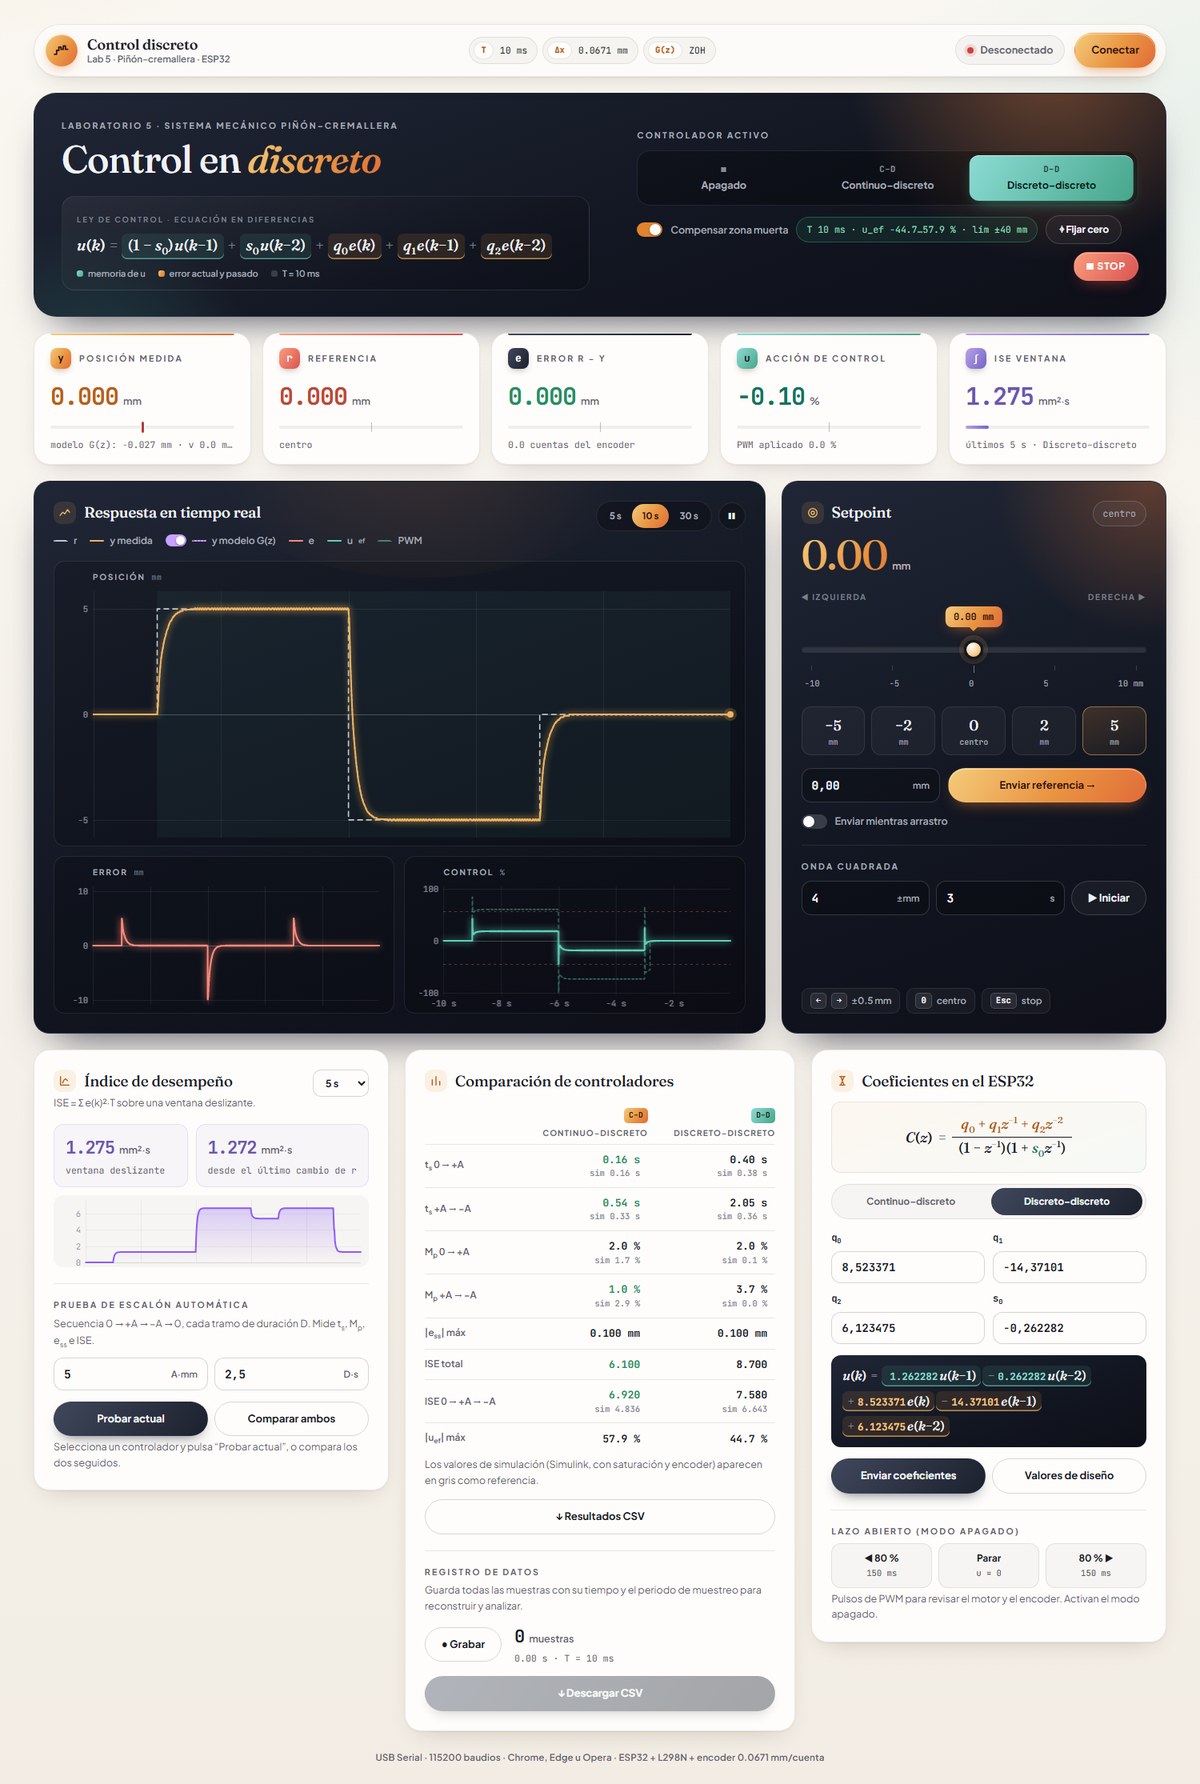
\includegraphics[width=0.6\textwidth]{interfaz_lab5_2.png}
  \caption{Interfaz gráfica: selector de controlador, indicadores, gráficas en
  tiempo real, setpoint, ISE, comparación de controladores y coeficientes.}
  \label{fig:app}
\end{figure*}

\begin{figure*}[!t]
  \centering
  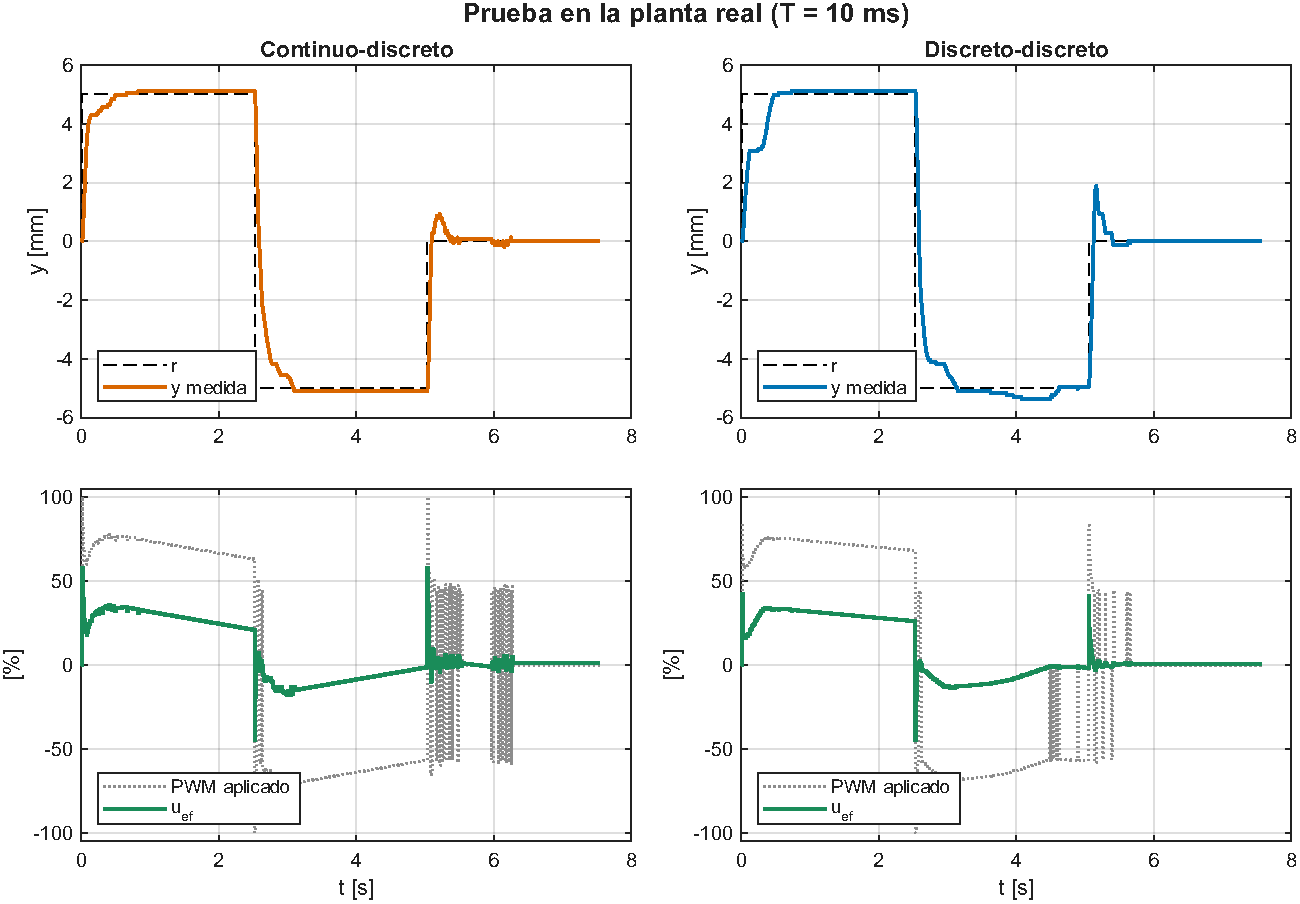
\includegraphics[width=0.85\textwidth]{real_lazo.pdf}
  \caption{Respuesta de la planta real con cada controlador: posición (arriba) y
  acción de control $u_{ef}$ y PWM aplicado (abajo).}
  \label{fig:real}
\end{figure*}

\subsection{Implementación en el ESP32}
El firmware (ESP-IDF) se organiza en dos tareas de FreeRTOS. La tarea de
control se despierta cada $T = 10$~ms con un retardo absoluto, de modo que el
periodo de muestreo no acumula error, y sigue el ciclo de la
Fig.~\ref{fig:flujo}: lee el encoder, calcula el error, evalúa la ecuación en
diferencias del controlador activo, (\ref{eq:ukcd}) o (\ref{eq:ukdd}), guarda
$u$ sin saturar en la memoria, satura $u_{ef}$ y le suma la zona muerta del
lado correspondiente antes de escribir el PWM. En el mismo ciclo evalúa la
ecuación en diferencias de la planta (\ref{eq:Gz}) para comparar el modelo
con la medición, revisa un límite de seguridad de posición y envía la
telemetría. La tarea de comandos atiende el puerto serie y cambia la
referencia, el controlador y sus coeficientes sin recompilar.

\begin{figure}[H]
  \centering
  \begin{tikzpicture}[
      node distance=1.6mm, font=\scriptsize, >={Stealth[length=1.6mm]},
      proc/.style={rectangle, draw, rounded corners=1pt, align=center,
                   text width=3.9cm, minimum height=4mm, inner sep=1.5pt, fill=blue!6},
      dec/.style={diamond, draw, aspect=2.4, align=center, inner sep=0.6pt,
                  fill=orange!12},
      term/.style={rectangle, draw, rounded corners=5pt, align=center,
                   text width=2.2cm, minimum height=4.6mm, fill=gray!15},
      side/.style={rectangle, draw, rounded corners=1pt, align=center,
                   text width=1.75cm, fill=green!8}]
    \node[term] (ini) {Inicio};
    \node[proc, below=of ini] (cfg) {Configurar PWM (1 kHz), encoder x4 y
      puerto serie; crear las tareas};
    \node[proc, below=of cfg] (esp) {Esperar el siguiente periodo $T = 10$~ms};
    \node[proc, below=of esp] (lee) {Leer encoder: $y(k) = \Delta x \cdot$ cuentas};
    \node[proc, below=of lee] (err) {$e(k) = r(k) - y(k)$};
    \node[dec, below=of err] (modo) {¿Lazo\\cerrado?};
    \node[proc, below=3mm of modo, text width=4.6cm] (ecu) {$u(k) = (1-s_0)u(k{-}1) + s_0u(k{-}2)$\\
      $+\,q_0e(k) + q_1e(k{-}1) + q_2e(k{-}2)$};
    \node[proc, below=of ecu] (mem) {Guardar $u(k)$ sin saturar ($\pm300$~\%)
      y desplazar $e$ y $u$};
    \node[proc, below=of mem] (sat) {$u_{ef} = \mathrm{sat}(u)$;\quad
      PWM $= u_{ef} + u_0^{\pm}$};
    \node[proc, below=of sat] (mod) {Modelo $G(z)$ y límite de seguridad de
      posición};
    \node[proc, below=of mod] (tx) {Enviar telemetría: $t$, $r$, $y$, $e$,
      $u_{ef}$, PWM, $v$, $y_{mod}$};
    \node[side, right=4mm of modo] (man) {Modo manual: PWM fijado por el
      usuario};
    \node[side, right=3mm of lee, dashed] (cmd) {Tarea de comandos: cambia $r$,
      controlador y coeficientes};

    \draw[->] (ini) -- (cfg);
    \draw[->] (cfg) -- (esp);
    \draw[->] (esp) -- (lee);
    \draw[->] (lee) -- (err);
    \draw[->] (err) -- (modo);
    \draw[->] (modo) -- node[left] {Sí} (ecu);
    \draw[->] (modo) -- node[above] {No} (man);
    \draw[->] (man) |- (mod.east);
    \draw[->] (ecu) -- (mem);
    \draw[->] (mem) -- (sat);
    \draw[->] (sat) -- (mod);
    \draw[->] (mod) -- (tx);
    \draw[->] (tx.west) -- ++(-3mm,0) |- (esp.west);
    \draw[->, dashed] (cmd.south) |- (err.east);
  \end{tikzpicture}
  \caption{Diagrama de flujo de la tarea de control del firmware.}
  \label{fig:flujo}
\end{figure}

\subsection{Interfaz gráfica}
La interfaz (Fig.~\ref{fig:app}) es una página web que se comunica con el
ESP32 por USB mediante Web Serial a 115200 baudios. Recibe cada muestra
($t$, $r$, $y$, $e$, $u_{ef}$, PWM, velocidad, salida del modelo y modo) y:
\begin{itemize}
  \item grafica en tiempo real la posición, el error y la acción de control;
  \item permite elegir el controlador y cambiar la referencia (deslizador,
        valores predefinidos, onda cuadrada y teclado);
  \item calcula el ISE $=\sum e(k)^2T$ sobre una ventana deslizante elegible
        (2--30~s) y desde el último cambio de referencia;
  \item ejecuta pruebas de escalón automáticas y compara $t_s$, $M_p$,
        $e_{ss}$ e ISE de ambos controladores junto a los valores simulados;
  \item guarda los datos en CSV con el tiempo de cada muestra y el periodo de
        muestreo en el encabezado, para su reconstrucción y análisis.
\end{itemize}

% ================= RESULTADOS =================
\section{Resultados y análisis}

Se aplicó a la planta real la secuencia de referencias
$0 \to 5 \to -5 \to 0$~mm con cada controlador (Fig.~\ref{fig:real}). Como el
2~\% de un escalón de 5~mm (0.1~mm) es menor que dos cuentas del encoder, el
tiempo de establecimiento se midió con una banda de $\pm0.134$~mm
(Tabla~\ref{tab:real}).

\begin{table}[H]
\centering
\caption{Resultados en la planta real (ISE en mm$^2\cdot$s)}
\label{tab:real}
\setlength{\tabcolsep}{3.5pt}
\resizebox{\columnwidth}{!}{%
\begin{tabular}{llccccc}
\toprule
 & Escalón & $t_s$ [s] & Sobrepico & $e_{ss}$ [mm] & ISE & $|u_{ef}|_{max}$\\
\midrule
\multirow{3}{*}{C--D} & $0\to5$  & 0.47 & 0.10 mm & $-0.10$ & 1.156 & 57.9\\
                      & $5\to-5$ & 0.53 & 0.10 mm & $+0.10$ & 5.769 & 44.7\\
                      & $-5\to0$ & 1.13 & 0.94 mm & $0.00$  & 0.889 & 57.9\\
\midrule
\multirow{3}{*}{D--D} & $0\to5$  & 0.45 & 0.10 mm & $-0.10$ & 2.336 & 42.6\\
                      & $5\to-5$ & 2.04 & 0.37 mm & $-0.03$ & 5.244 & 44.7\\
                      & $-5\to0$ & 0.35 & 1.88 mm & $0.00$  & 1.134 & 41.1\\
\midrule
\multicolumn{2}{l}{ISE total C--D} & \multicolumn{5}{l}{7.814}\\
\multicolumn{2}{l}{ISE total D--D} & \multicolumn{5}{l}{8.714}\\
\bottomrule
\end{tabular}}
\end{table}

\textbf{Estabilidad.} Los dos lazos fueron estables en todas las pruebas y
volvieron a la referencia después de cada escalón; los polos de lazo cerrado
de ambos diseños están dentro del círculo unitario (el D--D, exactamente en
$z = 0.875$ doble y $z = 0.513$ doble).

\textbf{Rapidez.} Hacia la derecha ambos se establecieron en
$\approx0.45$~s. En el escalón de $-10$~mm el C--D fue mucho más rápido
(0.53~s frente a 2.04~s): con $q_0 = 36.2$ satura el actuador al inicio y
empuja la masa con toda la autoridad disponible, mientras que el D--D, con
$q_0 = 8.5$, se acerca lentamente y queda atrapado por la fricción cerca de la
referencia hasta que la integral la libera (stick--slip). Ambos son más lentos
que en simulación porque el modelo lineal no incluye la fricción estática.

\textbf{Precisión.} En $\pm5$~mm el error final quedó en $\pm0.10$~mm
(1.5 cuentas): la fricción estática retiene la masa dentro de esa banda y la
integral crece despacio; en 0~mm el error fue nulo porque allí los resortes
están en equilibrio. El mayor sobrepico ocurrió al volver al centro
($0.94$ y $1.88$~mm): cerca de 0 los resortes casi no hacen fuerza y la
compensación de zona muerta, calculada con el equilibrio lejos del centro,
empuja de más.

\textbf{ISE.} El C--D acumuló menos ISE en total (7.81 frente a 8.71)
porque reduce el error más rápido en los escalones grandes; el D--D tuvo menos
ISE solo en el escalón de $-10$~mm (5.24 frente a 5.77), donde el C--D saturó
más tiempo. Con respecto a la simulación (4.84 y 6.64 para los dos primeros
escalones), el ISE real es mayor por la fricción, la zona muerta no ideal y el
juego del piñón, que el modelo no representa.

% ================= DISCUSIÓN =================
\section{Preguntas para la discusión}

\textbf{1. ¿Qué diferencias se observan entre los controladores diseñados
mediante las técnicas continuo--discreto y discreto--discreto?} El C--D parte
de un PID continuo y su desempeño depende de cuánto deforma la discretización
al lazo: con $p_3T = 1.33$ Euler introdujo 28.6~\% de sobrepico y fue
necesario reducir $p_3$. El D--D ubica los polos exactamente en el plano $z$,
incluye el retenedor y el cero de muestreo y dio ganancias cuatro veces
menores ($q_0 = 8.5$ frente a 36.2), con menos acción de control.

\textbf{2. ¿Cuál controlador presenta mejor desempeño según los criterios de
estabilidad, rapidez y precisión?} Ambos fueron estables y precisos dentro de
la resolución del encoder. En rapidez y en ISE total ganó el C--D; el D--D
exigió menos al actuador y fue más suave, pero sufrió más el stick--slip en el
escalón grande. Para esta planta con mucha fricción, el C--D tuvo el mejor
desempeño global.

\textbf{3. ¿Cómo se reflejan las diferencias entre controladores en el valor
del índice ISE?} El ISE castiga el error grande y sostenido: el controlador que
reduce antes el error (C--D) acumula menos ISE aunque sature, y el más lento
cerca de la referencia (D--D) acumula más. En simulación, el C--D tuvo
4.84 frente a 6.64 del D--D, y en la planta, 7.81 frente a 8.71.

\textbf{4. ¿Qué ventajas ofrece la implementación digital del controlador
mediante microcontroladores?} Los coeficientes se cambian por software sin
modificar el circuito (en la práctica 3 cada ganancia era una resistencia), se
pueden compensar no linealidades como la zona muerta, limitar la memoria del
integrador, cambiar entre controladores en caliente, ejecutar el modelo de la
planta en paralelo y registrar todas las señales; además no hay deriva de
componentes ni saturación de amplificadores operacionales.

\textbf{5. ¿Qué utilidad tiene la interfaz gráfica en el monitoreo y análisis
del sistema?} Permite ver en tiempo real la posición, el error y la acción de
control, detectar saturación o stick--slip, cambiar la referencia y el
controlador sin reprogramar, calcular el ISE sobre una ventana, comparar los
controladores con la misma prueba automática y guardar los datos con su tiempo
de muestreo para analizarlos después.

% ================= CONCLUSIONES =================
\section{Conclusiones}

\begin{itemize}
  \item La planta piñón--cremallera se representó con un modelo de segundo
        orden $G(s) = 168.4/(s^2 + 46.87s + 622.9)$ siempre que la entrada se
        exprese como PWM efectivo, descontando una zona muerta asimétrica
        (42.1~\% y 55.3~\%); sin esa corrección no hay un modelo lineal útil.
  \item El tiempo de muestreo de 10~ms cumplió los criterios de lazo cerrado y
        de Landau, y fue compatible con la resolución del encoder; la
        discretización ZOH calculada a mano coincidió con \texttt{c2d}.
  \item En la técnica continuo--discreto la ubicación del polo no dominante
        determinó si la discretización por Euler conservaba la respuesta:
        $p_3T \le 0.7$ fue necesario para no introducir sobrepico.
  \item Guardar la acción de control sin saturar en la memoria del controlador
        evitó que la masa se moviera en sentido contrario tras cada escalón.
  \item En la planta real ambos controladores siguieron la referencia con un
        error final de $\pm0.10$~mm; el C--D fue más rápido y con menor ISE total
        (7.81 frente a 8.71), y el D--D usó menos acción de control.
  \item Las diferencias entre simulación y experimento se explican por la
        fricción estática y el stick--slip, que el modelo lineal no incluye.
\end{itemize}

% ================= REFERENCIAS =================
\begin{thebibliography}{9}

\bibitem{ogata1995}
K. Ogata, \textit{Discrete-Time Control Systems}, 2nd ed. Prentice Hall, 1995.

\bibitem{ogata2010}
K. Ogata, \textit{Modern Control Engineering}. Prentice Hall, 2010.

\bibitem{franklin1998}
G. F. Franklin, J. D. Powell and M. L. Workman, \textit{Digital Control of
Dynamic Systems}, 3rd ed. Addison-Wesley, 1998.

\bibitem{landau2006}
I. D. Landau and G. Zito, \textit{Digital Control Systems: Design,
Identification and Implementation}. Springer, 2006.

\bibitem{kuo2009}
B. Kuo, \textit{Automatic Control System}. Wiley, 2009.

\bibitem{dorf2011}
R. Dorf, \textit{Modern Control Systems: International Version plus Matlab
and Simulink Student Version 2011a}. Pearson, 2011.

\bibitem{chen1993}
C. Chen, \textit{Analog and Digital Control System Design:
Transfer-Function, State-Space and Algebraic Methods}. Saunders College, 1993.

\bibitem{espressif2024}
Espressif Systems, \textit{ESP32 Series Datasheet}, Version 4.3, 2024.
[Online]. Available: https://www.espressif.com/en/support/download/documents

\end{thebibliography}

\end{document}
